\documentclass[a4paper,12pt,oneside]{book}
\usepackage[a-1b]{pdfx} % Creiamo un PDF/A per la consegna della tesi.
\linespread{1.5}
\usepackage{geometry}
\geometry{top=3cm,bottom=3cm,left=3.5cm,right=3.5cm} % Impostiamo il valore dei margini.
\usepackage[utf8]{inputenc}
\usepackage{tikz,pgf}
\usepackage{indentfirst}
\usepackage{amsfonts}
\usepackage[english]{babel} %% Abbiamo istruito LaTeX ad usare la lingua italiana.
\usepackage{todonotes}
\usepackage{subfig}
\usepackage{fancyhdr}
\setlength{\parindent}{1cm}
\usepackage{graphicx}
\usepackage{float}
\usepackage{csquotes}
\usepackage{amsmath}
\usepackage{numprint}
\usepackage{pgfplots}
\usepackage{pgfplotstable}
\usepackage{tocbibind}
\usepackage{tabto}
\usepackage{listings}
\usepackage{xcolor}
\definecolor{codegreen}{rgb}{0,0.6,0}
\definecolor{codegray}{rgb}{0.5,0.5,0.5}
\definecolor{codepurple}{rgb}{0.58,0,0.82}
\definecolor{backcolour}{rgb}{0.95,0.95,0.92}
\usepackage[ruled,linesnumbered,vlined]{algorithm2e}
\usepackage{amsthm}
\newtheorem{definition}{Definition}
\newtheorem{claim}{Claim}
\newtheorem{example}{Example}
\newtheorem{theorem}{Theorem}
\newtheorem{lemma}{Lemma}
\newtheorem{corollary}{Corollary}
\newcommand{\group}{\mathit{group}}
\newcommand{\lits}{\mathit{lits}}
\newcommand{\mwh}{\mathit{mwh}}
\newcommand{\wh}{\mathit{wh}}
\newcommand{\ml}{\mathit{ml}}
\newcommand{\inc}{\mathit{inc}}
\newcommand{\mps}{\mathit{mps}}
\newcommand{\blw}{\mathit{blw}}
\newcommand{\ext}{\xrightarrow{\text{ext}}}
\newcommand{\G}{\mathbb{G}}
\setlength{\parindent}{1cm}
\usepackage{graphicx}
\usepackage{float}
\usepackage{csquotes}
\usepackage{amsmath}
\usepackage{numprint}
\usepackage{pgfplots}
\usepackage{pgfplotstable}
\usepackage{tocbibind}
\usepackage{listings}
\setcounter{tocdepth}{3}
\usepackage{hyperref}
% \usepackage{algorithm}
% \usepackage{algorithmic}
\usepackage[
backend=biber,
style=ieee,
sorting=none
]{biblatex}
\addbibresource{references.bib}

\usepackage{fancyhdr}
\pagestyle{fancy}
\renewcommand{\headrulewidth}{0pt}
\fancyhf{}
\fancyhead[L]{}
\fancyfoot[C]{\thepage}
\def\amosum{\ensuremath{\textsc{amosum}}\xspace}


\graphicspath{{imgs/}} %% cartella dalla quale ricavare le immagini %%

\setlength {\marginparwidth }{2cm} 
\pgfplotsset{compat=1.16}

\newenvironment{dedication}
  {\clearpage           % we want a new page
   \thispagestyle{empty}% no header and footer
   \vspace*{\stretch{1}}% some space at the top 
   \itshape             % the text is in italics
   \raggedleft          % flush to the right margin
  }
   {\par % end the paragraph
   \vspace{\stretch{3}} % space at bottom is three times that at the top
   \clearpage           % finish off the page
  }
\lstdefinestyle{mystyle}{
    backgroundcolor=\color{backcolour},   
    commentstyle=\color{codegreen},
    keywordstyle=\color{magenta},
    numberstyle=\tiny\color{codegray},
    stringstyle=\color{codepurple},
    basicstyle=\ttfamily\footnotesize,
    breakatwhitespace=false,         
    breaklines=true,                 
    captionpos=b,                    
    keepspaces=true,                 
    numbers=left,                    
    numbersep=5pt,                  
    showspaces=false,                
    showstringspaces=false,
    showtabs=false,                  
    tabsize=2
}

\lstset{style=mystyle}
\usepackage{url}
\def\UrlFont{\rmfamily}
\usepackage{amsmath}
\usepackage{amssymb}
\usepackage{graphicx}
\usepackage{multirow}
\usepackage[ruled,linesnumbered,vlined]{algorithm2e}
\usepackage{booktabs}
\usepackage{url}
\usepackage{comment}
\usepackage{tikz}
\definecolor{darkgreen}{rgb}{0.0, 0.2, 0.13}
\definecolor{darkorange}{rgb}{1.0, 0.55, 0.0}
\definecolor{darkviolet}{rgb}{0.58, 0.0, 0.83}

\setlength {\marginparwidth }{2cm} 
\pgfplotsset{compat=1.16}
  
\begin{document}
%% Frontespizio %%
\begin{titlepage}
\begin{center}
\textbf{\LARGE Universit\`a della Calabria}\\
\textbf{Dipartimento di Matematica e Informatica}\\
\vskip 6pt
\hrule
\vskip 8pt

\includegraphics{logo.png}
\vskip 8pt
\textbf{Corso di Laurea Magistrale in\\ Artificial Intelligence \& Computer Science}
\vskip 32pt
Tesi di Laurea

\vskip 70pt
{ \huge \bfseries Design and Implementation of an AMO-SUM aggregate for ASP}\\[0.4cm]
\vskip 120pt

\begin{tabular}{p{8cm}p{8cm}}
Relatori: & Candidato:\\
Prof. Carmine Dodaro & Salvatore Fiorentino\\
Prof. Thomas Eiter & Matricola 242706\\
Dr. Tobias Geibinger & 
\end{tabular}

\vskip 60pt
\hrule
\vskip 6pt
Anno Accademico 2023/2024
\vfill
\end{center}
\end{titlepage}

% \usepackage{algorithm}
% \usepackage{algorithmicx}
% \usepackage{algpseudocode}

\begin{dedication}
Inserire dedica e ringraziamenti...
\end{dedication}

%% Corpo della tesi %%

%%\chapter*{Sommario} %% In questa zona inseriamo l'abstract del nostro documento. %%
%%Inserisci abstract: ...


\tableofcontents


\chapter*{Introduction}
\addcontentsline{toc}{chapter}{Introduction}
Answer Set Programming (ASP) is a highly utilized framework for knowledge 
representation and automated reasoning, as highlighted by \textit{Marek and Truszczyński (1999)} ~\cite{MarekT99}
and \textit{Niemelä (1999)} ~\cite{Niemela99}. 
In ASP, combinatorial problems are formulated using logical rules that incorporate various
linguistic constructs, which simplify the representation of complex knowledge.
In its most basic form, ASP programs consist of normal logic rules, where each rule 
has a head atom and a body that is a conjunction of literals. 
Often, normal programs are extended by incorporating aggregates, as discussed by 
\textit{Bartholomew et al. (2011)} \cite{DBLP:conf/aaaiss/BartholomewLM11}, \textit{Faber et al. (2011b)}
\cite{DBLP:journals/ai/FaberPL11}, \textit{Ferraris (2011)} \cite{DBLP:journals/tocl/Ferraris11},
\textit{Gelfond and Zhang (2014)} \cite{DBLP:journals/tplp/GelfondZ14},
\textit{Liu et al. (2010)} \cite{DBLP:journals/ai/LiuPST10},\textit{ and Simons et al. (2002)}
\cite{DBLP:journals/ai/LiuPST10}.
Specifically, \textit{SUM aggregates} are used in rule 
bodies, where literals are assigned weights, 
and the sum of the weights of the true literals must satisfy a specified (in)equality.
When the head of the rule is false the aggregate becomes a constraint aggregate.
Another kind of constraint is the \textit{At Most One} constraint
that essentially inhibits truth of pairs of literals in a given set.
It is very common that these two constraints (SUM and AMO) are linked together.
State of the art solvers treat this case ignoring the correlation between these two constraints. 
Our work aims to define a new costruct named \textit{AMO-SUM} to efficiently handle this case.
This efficiency improvement comes from the fact that we are able to treat the two constraint
as a whole constraint.

% The solutions to these problems are given in the form of stable models, 
% as described by \textit{Gelfond and Lifschitz (1990)} ~\cite{GelfondL90}. 
% In its most basic form, ASP programs consist of normal rules, where each normal rule 
% has a head atom and a body that is a conjunction of literals. 
% Intuitively, the head atom must be true whenever the associated body is true, 
% making stable models classical models of the propositional knowledge base created by
% translating normal rules into implications (body implies head). 
% The stability condition also ensures that stable models have additional properties, 
% such as being supported models (where every true atom is the head of some rule with a true body)
% as noted by \textit{Fages (1994)} ~\cite{DBLP:journals/mlcs/Fages94}, and unfounded-free models
% (where the support is acyclic) as described by 
% \textit{Dung (1992)} ~\cite{DBLP:journals/tcs/Dung92}.

% These properties are leveraged to achieve efficient computation by 
% integrating a conflict-driven clause learning 

Nowadays current ASP solver implements a (CDCL) algorithm with propagators, 
as explained by \textit{Gebser et al. (2012)} ~\cite{DBLP:journals/ai/GebserKS12}.
CDCL (Conflict-Driven Clause Learning) is a contemporary form of non-chronological 
backtracking that follows the \textit{choose-propagate-learn} pattern, 
as described by \textit{Marques-Silva et al. (2021)} ~\cite{DBLP:series/faia/0001LM21}, ~\cite{DIMCAS}.

% The \textbf{choose} phase, or decision phase, consists in the process
% of \textit{choosing} a (branching) literal as the new literal to become true.
% After a literal has been choosed the so-called \textbf{propagate} phase takes place, whose role 
% is to extend the current partial assignment: a partial assigment
% is a non-total function on the atoms of the program that maps each of them to a boolean value.
% Extending means mapping literals to boolean value that can be deterministically inferred from the
% program and the current partial assignment. Specifically, process propagate employs a series of propagation functions,
% often referred as \textit{propagators}, following a priority sequence.
% The \textbf{learn} phase occurs when a conflict is detected, that is when the partial assignment contains a contradiction.
% In this stage a new clause has to be learned, to not make the same mistake again.
% To learn this clause each inferred literal is linked to a reason, which is a clause (a set of literals)
% that led to derived the literal in the propagation phase.
% When conflicts arise, these reasons are used to learn new clauses,
% effectively pruning the search space and enhancing the efficiency of the search process.
This pattern consists of this three phases: 
\textbf{choose} phase, or decision phase, consists in picking a branking literal as true; 
\textbf{propagate} phase derives determinists consequences of the current state;
\textbf{learn} phase is triggered when a conflict arises and aims at understanding from the conflict 
to not making the same mistake again.
In the propagate phase  specific procedures called \textit{propagators} are used to derive such consequences.
Propagators are required to explain why a consequence has been derived.
This explanation is called reason, it is a set of literals that led to derive that consequence 
and it is used in the learning phase.
When an aggregate is introduced inside the program then a specific propagator is required.
Our work provides both a novel propagator for handling the new AMO-SUM construct and 
an algorithm to minimize the reasons of the aggregate-derived consequences.
To provide a more comprehensive understanding of our work the \todo{DA FINIRE}





\chapter{Background}

This chapter defines all the background needed to explain our work,
trying to guide the reading through a clear and intuitive idea.
Initially the syntax and semantics of normal
program (section $~\ref{sec:bg-syntax_semantics}$) is showed,
primarly focusing on notions relevant for this thesis, for instance on some
extension such as the SUM constraints.
Then some specific cases of SUM constraints, the so-called ALO and AMO constraints, 
is explained in section $~\eqref{sec:bg-clauses_AMO}$.
Afterwards, the current state-of-the-art ASP solver algorithm to find a stable model 
is discussed (section $~\ref{sec:bg-SM}$), focusing on the concept of \textit{propagator}.

\section{Syntax and Semantics}
\label{sec:bg-syntax_semantics}

This section proceeds in a bottom-up fashion, introducing the 
most basic elements to the concept of \textit{program}
and \textit{stable model}.

The first element is the set of \textit{atoms}, let $\mathcal{A}$ be such set.
$\neg$ is a symbol representing the common negation in logic.
A $\emph{literal}$ is an atom with possibly the negation symbol in front of it.
For instance $a \in \mathcal{A}$ is a literal (and an atom) and $\neg b$ with $b \in \mathcal{A}$
is a literal (but not an atom); \textit{a} is said to be a \textit{positive literal} instead
$\neg b$ is a negative literal. In a more formal way: given a literal $\ell \in L$, $\ell$ is 
positive if $\ell \in \mathcal{A}$ otherwise it is negative. Let $L$ be a set of literals.
Given $\ell \in L$ then $\overline{\ell}$ denotes its complement, if $\ell$ is a positive
literal, i.e. $\ell = a \in \mathcal{A}$, then $\overline{\ell} = \neg a$ else 
when $\ell = \neg a$ (negative literal) with $a \in \mathcal{A}$ then $\overline{\ell} = a$.
A set of literal $L$ can be negated, written $\overline{L}$;
$\overline{L}$ is equivalent to the set of literals of $L$ where each literal is negated,
that is, $\overline{L} = \{ \overline{\ell} \mid \ell \in L \}$.

Each atom can be mapped to a truth value (boolean value) by an \textit{intepretation}.
An \textit{intepretation} (or \textit{assignment}) \textit{I} is a set of 
literals where $I \cap \overline{I} = \emptyset$.
If $\mathcal{A} \subseteq (I \cup \overline{I})$ then $I$ is called \textit{total-intepretation},
otherwise it is a \textit{partial-intepretation}.
On one hand if $\ell \in I$ then $\ell$ is \textit{true} under $I$, on the other hand 
if $\ell \in \overline{I}$ then it is \textit{false} under $I$.
If either $\ell \not\in I$ and $\ell \not\in \overline{I}$ then $\ell$ is said to be \textit{undefined}. 
Abusing of notation, If $\ell \in I$ let $I^{\top}(\ell) := 1$, 0 otherwise;
if $\ell \not\in \overline{I}$ let $I^{\neg\bot}(\ell) := 1$, 0 otherwise.

Now the first main brick can be presented: the rule.
A rule is a classic implication in propositional logic.
\begin{align}\label{eq:rule}
    r: \quad p \leftarrow \ell_1, \ldots, \ell_n
\end{align}
where \textit{p} is an atom and $\ell_1, \ldots, \ell_n$ with $n \ge 0$ are literals.
The rule r  $~\ref{eq:rule}$ is equivalent to $\ell_1 \land\, \ldots \, \land  \ell_n \rightarrow p$.
As in propositional logic $p$ and $\ell_1, \ldots, \ell_n$ are named respectively \textit{head}
and \textit{body} of the rule.
The head of \textit{r} is defined by the symbol $\mathit{H}(r) := p$
and the body by the set
$\mathit{B}(r) := \{\ell_1, \ldots, \ell_n \}$.
Each rule has a \textit{positive} and \textit{negative} part, and it is stricly 
linked with the concept of positive and negative literal.
On one hand, the positive body of the rule \textit{r}, named $\mathit{B}^+(r)$, is the set
of positive literals of \textit{r}, that is, 
$\mathit{B}^+(r) = \{ \ell \mid \{\ell\} \cap \mathcal{A} \ne \emptyset \}$.
On the other hand, the negative body of the rule \textit{r}, named $\mathit{B}^-(r)$, is the set
of negative literals of \textit{r}, namely, 
$\mathit{B}^-(r) = \{ \ell \mid \{\ell\} \cap \mathcal{A} = \emptyset \}$

Now the relation $\models$ (satisfies, or is model of) is inductly 
defined: let $I$ be an intepretation, if $\ell \in I$ then $I \models \ell$;
if $\ell \in \overline{I}$ then $I \models \overline{\ell}$;
if $I \models \ell_+$ for every $\ell_+ \in B^+(r)$ and 
$I \models \ell_-$ for every $\ell_-\in B^-(r)$, then $I \models B(r)$;
if whenever $I \models B(r)$ also $I \models H(r)$ then $I \models r$.
A (normal) program $\Pi$ is a set of rules.
$M(\Pi) = \{ I \mid I \models \Pi\}$ is the set of \textit{models} of $\Pi$. 

Let's now shift to another concept that allow us to 
transition from a normal program to an extension of it: the concept of \textit{SUM constraint}.
A SUM constraint (or simply constraint) has the following form
\begin{align}\label{eq:sum}
    \textsc{sum}\{w_1 : \ell_1;\ \cdots;\ w_n : \ell_n\} \geq b
\end{align}
where $n \ge 0$, $\{\ell_1, \hdots, \ell_n\}$ is a set of literals such that 
$\ell_i \ne \ell_j$ for all $i,j \in \{1, \hdots, n\}$ such that $i \ne j$
and $\{b, w_1, \hdots, w_n \}$ is a set of naturals numbers.
Let $\sigma$  be a constraint of the form $~\ref{eq:sum}$ then $\mathit{bnd}_{\sigma} = b$
represents the \textit{bound} of the constraint $\sigma$; $w_1, \hdots, w_n$
are the weights of each literal in $\sigma$; $lits_{\sigma}$ is the set of literals of $\sigma$.
Let's specify the relation $\in$ as $(w_i, \ell_i) \in \sigma$ to be read  
as $(w_i : \ell_i)$ is an element in (the aggregation set of) $\sigma$;
The function $\mathit{wh_{\sigma}}(\ell_i) = w_i$, namely, this is a function that 
maps every literal of $\sigma$ to its weight.
Intuitively, the constraint is satisfied w.r.t. an interpretation $I$ 
if summing the weight of the true literals under $I$ yields to value greater or equal to the bound.
More formally, extending the relation $\models$, $\sigma$ is satisfied if 
$\sum_{i=1}^{n} \mathit{wh}_{\sigma}(l_i) \cdot I^{\top}(l_i) \ge \mathit{bnd}_{\sigma}$,
written $I \models \sigma$.
Note that $\sigma$ may be omitted from the above notation if its meaning is clear from context.\\
Just as a side note: in ASP-Core-2 standard
~\cite{DBLP:journals/tplp/CalimeriFGIKKLM20} 
the constraint  $~\ref{eq:sum}$ is written as the headless rule
$\mathit{:-} \quad \#sum\{w_1,\ell_1 : \ell_1; ...; w_n,\ell_n : \ell_n\} < b.$
Now a more formal definition of program can be given:
a program $\Pi$ is a set of rules and constraint, referred as $\mathit{rules}(\Pi)$ 
and $\mathit{constraints}(\Pi)$ respectively.
The sets of rules and constraints define the set of atoms of the program and they are named $\mathit{atoms}(\Pi)$.
Finally, $I$ satisfies $\Pi$, written $I \models \Pi$, if $I \models r$ for all $r \in \mathit{rules}(\Pi)$
and $I \models \sigma$ for all $\sigma \in \mathit{constraints}(\Pi)$.

To make the discussion made so far more understandable, we will introduce the following example:
\begin{example}[Running example]
    \label{ex:running}
    Let $\Pi_{\mathit{run}}$ be the following:
    \begin{align*}
        \begin{array}{rll}
            r_{\alpha\phantom{'}}: & \alpha\phantom{'} \leftarrow \neg \alpha' & \alpha \in \{x,y,z\}\\
            r_{\alpha'}: & \alpha' \leftarrow \neg \alpha & \alpha \in \{x,y,z\}\\ 
            \sigma_{1}: & \textsc{sum}\{
                1 : \overline{x};\ 1 : \overline{y}\phantom{;\ 2 : z}
            \} \geq 1 \\
            \sigma_{2}: & \textsc{sum}\{
                1 : x;\ 2 : y;\ 2 : z
            \} \geq 3
        \end{array}
    \end{align*}
Note that there are six atoms ($x,y,z,x',y',z'$), six rules and two constraints.
$\mathit{wh}_{\sigma_1}(\overline{x}) = 1, \mathit{wh}_{\sigma_1}(\overline{y}) = 1,
\mathit{wh}_{\sigma_2}(x) = 1,\mathit{wh}_{\sigma_2}(y) = 2,
\mathit{wh}_{\sigma_2}(z) = 2, \mathit{bnd}_{\sigma_1}=1,\mathit{bnd}_{\sigma_2}=3$.
\end{example}
A possible (total) interpretation $I$ satisfying $\Pi_{\mathit{run}}$ is:
$I_1 = \{ x, z, \overline{y}, x', y', z' \}$.
Since, $\sum_{i=1}^{2} \mathit{wh}_{\sigma_1}(\ell_i) \cdot I_1^{\top}(\ell_i) = 
\sum 1 \cdot I_1^{\top}(\overline{x}) + 1 \cdot I_1^{\top}(\overline{y}) = 1 \ge \mathit{bnd}_{\sigma_1}$
and $1 \cdot I_1(x) + 2 \cdot I_1^{\top}(y) + 2 \cdot I_1^{\top}(z) = 3 \ge \mathit{bnd}_{\sigma_2}$.
Given a program $\Pi$ and an intepretation $I$, its \textit{reduct} is
defined as follows: $\Pi^{I} = \{ H(r) \leftarrow B^+(r) \mid r \in \mathit{rules}, I \models B(r)\}$,
please note that $\mathit{constraints}(\Pi^{I}) = \emptyset$.
One interpretation may differ from another due to its stability.
An interpretation $I$ is a stable model of a program $\Pi$ if $I \models \Pi$ and there is 
no $J \subset I$ such that $J \models \Pi^I$ .
Let $\mathit{SM}(\Pi)$ denote the set of stable models of $\Pi$.
Taking in consideration example $~\ref{ex:running}$ we can notice that 
$I_1$ is not a stable model, that is, $I_1 \not\in \mathit{SM}(\Pi_{\mathit{run}})$.
This is because taking the partial assignment $J_1 = \{y'\}$
then $ J_1  \models \Pi_{\mathit{run}}^{I_1}$ since $\Pi_{\mathit{run}}^{I_1} = \{ y' \leftarrow  \}$
and $J_1 \subset I_1$.
Instead $I_2 = \{ x, z, \overline{y}, \overline{x'}, y', \overline{z'} \} \in \mathit{SM}(\Pi_{\mathit{run}})$.

Continuing talking about the above example, a last consideration that let us to move towards the next 
chapter has to be addressed.
The constraint $\sigma_1$ is a special one, it says: at least 1 of the 2 literals
has to be satisfied. Notice that all the literals are flipped, 
so referring to the literals without being flipped it is 
actually saying `at least 1 of the 2 have to be falsified' , and since $2 = 1 - 1$ it can be 
reformulated as 'at most 1 of them can be satisfied'.
Thus, with an \textit{At least One (ALO)} sum constraint is possible to define an \textit{At Most One (AMO)}
constraint.

\section{ALO (clauses) and AMO as a Special Case}
\label{sec:bg-clauses_AMO}

Given a set $\{\ell_1, \hdots, \ell_n\}$, with $n \ge 1$, an \textit{At Least One (ALO)} 
constraint over this set will enforce to have at least one literal true.
As in the example $~\ref{ex:running}$ it can be expressed as:
\begin{align}\label{eq:ALO}
    \textsc{sum}\{1 : \ell_1;\ \cdots;\ 1 : \ell_n\} \geq 1
\end{align}
This constraint can be written as a \textit{set} of the form 
\begin{align}
    \label{eq:clauses}
    \{\ell_1, \hdots, \ell_n\}
\end{align} 
Usually this constraint is named also \textit{clause} (following the \textit{CNF} notation 
of the propositional logic).
Modern ASP solvers enrich the input program with clauses enforcing $I$ to be a 
model of rules of the form \eqref{eq:rule} (i.e., $\{p, \overline{\ell_1}, \ldots, \overline{\ell_n}\}$).
If over this set instead is enforced an \textit{At Most Constraint}, i.e., at most 
one literal is true, the following constraint is introduced:
\begin{align}\label{eq:amo}
    \textsc{sum}\{1 : \overline{\ell_1};\ \cdots;\ 1 : \overline{\ell_n}\} \geq n - 1
\end{align}
To enforce that at most
one literal is true of a given set it is enough to enforce that 
at least $n-1$ literals are falsified.
Since, intuitively, if two different literals are satisfied then $n-2$ literals are not falsified.
More formally given an interpretation $I$, $I$ satisfies at most 1 literal if 
$\sum_{i = 1}^{n}{I^{\top}(\overline{\ell_i})} \geq n - 1$, or equivalently
$\sum_{i = 1}^{n}{I^{\top}(\ell_i)} \leq 1$.
The AMO constraint \eqref{eq:amo} is compactly written $\textsc{amo}\{\ell_1,\ldots,\ell_n\}$.
\begin{example}[Continuing Example~\ref{ex:running}]
    Note that $\sigma_1$ is the clause $\{\overline{x}, \overline{y}\}$, or also the AMO constraint $\textsc{amo}\{x, y\}$.
\end{example}
\section{Stable Model Search, Propagators and Learning}
\label{sec:bg-SM}

Currently ASP solvers employ a \textit{conflict-driven clause learning} (CDCL) algorithm
\cite{DBLP:journals/ai/GebserKS12} to search a stable model.
This is an algorithm also used in a lot of SAT solvers and it has been revealed to be a 
very effective one.
The CDCL follows a pattern called \textit{choose-propagate-learn}, where: 
the \textit{choose} phase consists in deciding a literal to become true, such literal 
is named \textit{branching literal};
\textit{propagate} phase involves to deterministically derive new consequences from the current
state (interpretation); \textit{learn} phase, when a conflict arises, understands
some new \textit{clause} (constraint) that was not explicity defined in the program.
To dive into each of these phases, understanding the CDCL, some previous concepts have
to be mentioned.

A \textit{conflict} occurrs in an intepretation $I$,
when two literals $\ell, \overline{\ell}$ are together in $I$.
Given two clauses $C,D$ of the form \eqref{eq:clauses} (as described in $~\ref{sec:bg-clauses_AMO}$) and a literal 
$\ell$ such that $\ell \in C$ and $\overline{\ell} \in D$ then the \textit{resolution}
(~\cite{davis1960computing}, ~\cite{robinson1965machine})
step of $C$ and $D$ upon $\ell$, written $C \otimes_{\ell} D$, is equal to 
$(C \setminus \{\ell\}) \cup (D \setminus \{\overline{\ell}\})$.
Intuitively, if $C \in \Pi$ and $D \in \Pi$ 
then since an intepretation cannot simultaneously
satisfying $\ell$ and $\overline{\ell}$ then $C \setminus \{\ell\}$ or 
$D \setminus \{ \overline{\ell}\}$ have to be satisfied, thus the following clause 
$(C \setminus \{\ell\}) \cup (D \setminus \overline{\ell})$ has to be satisfied.
Please note that if an intepretation $I \models \Pi$ then $I \models C \otimes_{\ell} D$.
So $C \otimes_{\ell} D$ is implied by the program,
written $\Pi \models C \otimes_{\ell} D$.
A clause $C$ is \textit{redundant} in $\Pi$ if $\Pi \models C$.
Given a clause $C$ then an assignment $I$ that \textit{blocks}
$C$ is an assignment that falsifies all literals (and no others)
of $C$, i.e., $I = \overline{C}$. 

In the \textit{choose} phase a branching (undefined) literal is selected.
Every branching (or decision) literal is paired with a \textit{decision level}.
To understand the decision level is enough to 
now that at each choose phase the corresponding literal is added into a 'list' and
the decision level is the index into the list (index starting from 1). 
The term `\textit{backjumping} to a certain level $l$' refers to the process of `forgetting' 
every decision made after decision level $l$, 
including the respective propagated literals, and then 
resuming the decision-making process starting from level $l$.


In the \textit{propagate}, given an intepretation $I$,
potentially some literal $\ell$ is derivated 
(or propagated) using a \textit{Propagate} function according to some \textit{inference rule}.
An inference rule is a logical construct used  
to derive new \textit{literals} (\textit{conclusions}) 
from a current intepretation $I$ (\textit{premises}). 
It specifies the conditions under which certain statements (the conclusions) 
can be inferred from other statements (the premises).
After a literal $\ell$ is inferred, thanks to some inference rule, then a \textit{reason}, written $\mathit{reason}(\ell)$, 
is specified. This reason defines \textit{why} $\ell$ has been propagated.
More in detail, the reason is a clause of this form 
\begin{align}
    \label{eq:reason_form}
    R = \{ \ell \} \cup \{\overline{\ell_1},\hdots, \overline{\ell_n}\}
\end{align}
\eqref{eq:reason_form} represents the implication 
rule $\ell_1 \land \hdots \land \ell_n \rightarrow \ell$ and it specifies 
that when all the literals $\ell_1 \land \hdots \land \ell_n$ are true then also 
$\ell$ must be true. $B(R) = \overline{\{\overline{\ell_1},\hdots, \overline{\ell_n}\}}$
is the body of the reason and $H(R) = \{\ell\}$.
$R$ is said to be a reason of the literal $z$ if $H(R) = \{z\}$.
$J_R= B(R)$ is the assigment satisfying the body of $R$; note that $J_R$ is blocking $R \setminus H(R)$.
A clause $C$ of the form \eqref{eq:reason_form} is a reason for $\ell$, under the assignment $I$, 
if $I \supseteq B(C)$ and under intepretation $J_c$ the propagator 
infers  $\ell$, thanks to some inference rule.
Finally, $\mathit{reason}(\ell)$ has to be a reason of $\ell$ under $I$.
Can happen that inferring a literal $\ell$ creates a conflic (i.e., $\overline{\ell} \in I$),
in that case $\ell$ is a \textit{conflict literal}.
Moreover $\ell$ is also paired with a decision literal 
that it is inherited from the current decision level of the search.
\textit{Unit Propagation} is a specific kind of propagation, it is applied when given a clause 
$C$ and a literal $\ell \in C $, $(C \setminus \{\ell\}) \cap \overline{I} = C \setminus \{\ell\}$.
In this case the only way to satisfy $C$ is setting $\ell$ to true, thus $\ell$
is propagated to true; the reason is exactly because the other literals are falses, so 
$reason(\ell) = C$.
Please not the $reason(\ell)$ respresents $\overline{\ell_1} \land \hdots \land \overline{\ell_n} \rightarrow \ell$, where 
$\{\ell_1 \land \hdots \land \ell_n\} = C \cap \overline{I}$.The \textit{Propagate} function is implemented using multiple \textit{propagators},
calling them sequentially according to a priority list.

The whole algorithm, initially starts with an empty assignment (all literals undefined)
and a the decision level (\textit{dl}) to 0  ,
then the \textit{propagate} phases takes place, inferring all the consequences.
If a conflict is detected it means that the program is not satisfiable, since 
without any choice we got a conflict.
Else, if no conflict is detected then the \textit{choose} phase decides the new branching literal.
An important note is that just the a branching literal $\ell$ has a reason of the form $\{\ell\}$, representing
$\rightarrow \ell$ ($\ell$ must be true), since it 
does not follows from any logic reasoning.
Then, again the propagate phase is executed.
If a conflict is detected then a process named \textit{conflict analysis} starts.
Starting from the reason of the conflict literal a (\textit{backward}) resolution upon a literal of the last
decision level is perfomed. This step is iteratively done until the new obtained (redundant) clause 
contains just one literal of the current decision level, this clause in called
\textit{Unique Implication Point (UIP)}.
Given the UIP then a \textit{backjump} operation is perfomed to the second highest decision level
(\textit{assertion level}); to update the internal state following a backjump, the \textit{Unroll}
function is invoked for each propagator.
The assertion level is special in the sense that it is the deepest level
at which adding the conflict-driven clause (UIP) would allow unit propagation to derive
a new implication using that clause. Since the literal with highest dl after backjumping 
is the only undefined literal inside UIP then the unit propagation will infer that literal,
that is, will flip the previous value.
When the highest literal in the UIP has 0 as dl then the assertion level is -1 by default.
Some \textbf{important} final notes: the reason for a literal $\ell$
must include at least one literal from the most recent decision level, excluding $\ell$
itself, otherwise, unit propagation 
cannot be performed; the smaller the cardinality of the conflict literal's reason, 
the higher the potential jump in the search space.
After this, a new choice is made until either all atoms are defined or the
assertion level is -1.
The above described algorithm is defined below and it is mainly based on the algorithm 
defined in \cite{DBLP:series/faia/SilvaLM09}.
\begin{algorithm}[h]\small
    \caption{Typical CDCL algorithm}
        \label{alg:cdcl}
        \SetKwInOut{Input}{Input}
        \Input{An ASP program $\Pi$}
        \SetKwBlock{Loop}{Loop}{end}
        \Begin{
            $I \gets [\,]$\\
            $dl \gets 0$\\
            \If {(\textsc{Propagate}$(\Pi, I) == \text{CONFLICT}$)}{
                \Return{Unsat}
            }
            \While{\textsc{not} \textsc{AllVariablesAssigned}$(\Pi, I)$}{
                $\ell = \textsc{PickBranchingLiteral}(\Pi, I)$ \\
                $dl \gets dl + 1$ \\
                $\mathit{store}(I,\ell,dl)$\\
                \If {(\textsc{Propagate}$(\Pi, I) == \text{CONFLICT}$)}{
                    $\beta = \textsc{ConflictAnalysis}(\Pi, I)$\\         
                    \If {($\beta < 0$)}{
                        \Return{Unsat}
                    }
                    \Else{
                        \textsc{Backjump}$(\Pi, I, \beta)$\\
                        $dl \gets \beta$ \\
                    }
                }
            }
        \Return{I}
        }
        
\end{algorithm}

Let's assume for now that the Propagate function is exactly equal to the propagator
implementing \textit{Unit propagation},
this is usefull for the next example.

\begin{example}\label{ex:unit-propagation}
    Let $\Pi$ have, among others, the rules
    \begin{align*}
        \begin{array}{ccc}
            x \leftarrow \neg z \qquad &
            y \leftarrow \neg z \qquad &
            w \leftarrow x, y
        \end{array}
    \end{align*}
    Hence, a modern ASP solver materializes the clauses
    \begin{align*}
        \begin{array}{ccc}
            \{x,z\} \qquad &
            \{y,z\} \qquad &
            \{w,\overline{x},\overline{y}\}
        \end{array}
    \end{align*}
    For readability at each literal is associated the relative decision level 
    as superscript.
    Let's assume that the current interpretation is 
    $I = [\overline{w}^1]$ and the decision level is $dl= 1$.
    Since no propagation is performed the algorithm goes 
    directly to the propagate phase, let's assume that 
    $\overline{z}$ is selected.
    Then, by unit propagation, $x$ and $y$ are inferred,
    thanks to the first two clauses.
    Unit propagation infers $x, y$ from the first two clauses, and then $y$ 
    (a conflict literal) from the third clause.
    The correspective reasons are: $reason(x) = \{ x, z \}$,
    $reason(y) = \{ y, z \}$ and $reason(\overline{y}) = \{w,\overline{x},\overline{y}\}$.
    The current intepretation $I$ is equal to
    $[\overline{w}^1,\overline{z}^2, y^2, x^2]$.
    Since there are more than 1 literal of the decision level 2 (the last one) in the conflict clause
    ($\{w,\overline{x},\overline{y}\}$)
    a backward resolution step is perfomed.
    Let's take arbitrarily $\overline{x}$:
    $\{w,\overline{x},\overline{y}\} \otimes_{\overline{x}} \{ x, z \}= \{w, \overline{y}, z\}$.
    Since both $\overline{y}, z$ are with decision level 2 then let's take arbitrarily $\overline{y}$:
    $\{w, \overline{y}, z\} \otimes_{\overline{y}} \{y,z\} = \{w, z, z\} = 
    \{w, z\}$.\\
    $\{w, z\}$ is \textit{UIP} so let's backjump to the assertion level 1.
    This will unit propagate $z$ with $reason(z) = \{w, z\}$.
    So the intepretation will look like: $I = [\overline{w}^1, z^1]$
\end{example}

The main difference between a SAT solver and a ASP solver can be summarized focusing on 
the function $\mathit{Propagate}(\Pi,I)$.
SAT solvers employ mainly unit propagation inside the \textit{Propagate} function,
instead ASP solvers use, in addition on unit propagation, other two fundamental  
propagation functions: \textit{Unfounded-free propagation} and \textit{ConstraintPropagation}.
The first one (\textit{Unfounded-free propagation}) assesses that the intepretation is a stable model, but its details
are out of the scope of this work.
The second one (\textit{ConstraintPropagation}) is used to derive new consequences from 
the constraints present in the program. 
For a SUM constraint $\sigma$ of the form \eqref{eq:sum},
solvers typically employ a 
specific \textit{constraint propagator}
~\cite{DBLP:conf/iclp/GebserKKS09,DBLP:journals/fuin/FaberLMR11} leveraging the concept of 
\textit{max possible sum (mps)}.
Given an intepretation $I$, a literal $\ell$ and a constraint $\sigma$ of the form \eqref{eq:sum}, 
a max possible sum, considering $\ell$ as false, is $\mathit{mps}_{\sigma}(I,\ell) = 
\sum_{j \in [1..n], \ell_j \neq \ell}{w_j \cdot I^{\neg\bot}(\ell_j)}$;
intuitively, if all the undefined literal were true and $\ell$ was false
then the sum would be equal to $\mathit{mps}_{\sigma}(I,\ell)$.
An inference rule of a sum constraint essentially adds to $I$ the literal $\ell$ 
if $\ell$ is required to (possibly) reach the bound $b$, i.e., if
\begin{align}\label{eq:sum:propagation}
    \mathit{mps}_{\sigma}(I,\ell) < \mathit{bnd}_{\sigma}
\end{align}
In this case \textit{reason}$(\ell) = \{\ell\} \cup lits_{\sigma} \cap \overline{I}$.
A rational behind this is as follows: if in the best case (that is, when the sum is $\mathit{mps}(I,\ell)$)
the sum does not reach the bound it means that $\ell$ cannot be false, that is, it is required to be true.
Intuitively, the falses literals are the only justification why the bound $\mathit{bnd}_{\sigma}$
could be not reached if $\ell$ was not added to $I$.
In the special case of \eqref{eq:amo}, that is, if $\sigma$ is $\textsc{amo}\{\ell_1, \ldots, \ell_n\}$, the literal $\overline{\ell}_i$ ($i \in [1..n]$) is added to $I$ if there is $\ell_j$, with $j \neq i$, such that $\ell_j \in I$.
In this case, $\mathit{reason}(\overline{\ell_i})$ is $\{\overline{\ell_i}, \overline{\ell_j}\}$.

\begin{example}[Continuing Example ~\ref{ex:running}] \label{ex:sumpropagator}
    If $I$ is empty, no literal can be inferred from $\sigma_1$ and $\sigma_2$.
    If $I$ is $[\overline{z}]$, then the application of \eqref{eq:sum:propagation} to the literals of $\sigma_2$ gives
    \begin{align*}
        2 \cdot [\overline{z}]^\uparrow(y) + 2 \cdot [\overline{z}]^\uparrow(z) = 2 \cdot 1 + 2 \cdot 0 = 2 < 3\\
        1 \cdot [\overline{z}]^\uparrow(x) + 2 \cdot [\overline{z}]^\uparrow(z) = 1\cdot 1 + 2 \cdot 0 = 1 < 3\\
        1 \cdot [\overline{z}]^\uparrow(x) + 2 \cdot [\overline{z}]^\uparrow(y) = 1 \cdot 1 + 2 \cdot 1 = 3 \not< 3
    \end{align*}
    Hence, $x$ and $y$ are inferred with
    $\mathit{reason}(x) = \{x,z\}$ and
    $\mathit{reason}(y) = \{y,z\}$.
    Note that, once $I = [\overline{z},x,y]$, the application of \eqref{eq:sum:propagation} to $\sigma_1$ gives
    \begin{align*}
        1 \cdot [\overline{z},x,y]^\uparrow(\overline{y}) = 1 \cdot 0 = 0 < 1\\
        1 \cdot [\overline{z},x,y]^\uparrow(\overline{x}) = 1 \cdot 0 = 0 < 1
    \end{align*}
    Therefore, a conflict is raised, say because $\overline{y}$ (or similarly $\overline{x}$) 
    is added to $I$ with $\mathit{reason}(\overline{y}) = \{\overline{x}, \overline{y}\}$.
\end{example}

\chapter{AMOSUM}
\label{cp:AMOSUM}
In this chapter we propose a new constraint with 
relative syntax and semantics (section ~\ref{sec:amo:syntax_semantics}).
This constraint combines a SUM constraint of the form  \eqref{eq:sum} 
with a collection of AMO constraints of the form \eqref{eq:amo}.
Then the related rules for propagating are described in section ~\ref{sec:amo:inference_rules}.
Finally the \textit{Propagate} and the \textit{Unroll} functions are defined 
in the last two sections

\section{Syntax and Semantics}
\label{sec:amo:syntax_semantics}
An \textit{AMOSUM} constraint is defined as follows:
\begin{align}\label{eq:amosum}
    \amosum\{w_1 : \ell_1\ [g_1];\ \cdots;\ w_n : \ell_n\ [g_n]\} \geq b
\end{align} 
where $n \geq 0$, $\ell_1,\ldots,\ell_n$ are distinct literals such that $\ell_i \neq \overline{\ell_j}$ (for all $1 \leq i < j \leq n$),
and $b,w_1,\ldots,w_n,g_1,\ldots,g_n$ are naturals numbers. 
As in \eqref{eq:sum}: $\{w_1,\ldots,w_n\}$ is the set of weights and $\mathit{wh}_{\sigma}(l_i) = w_i$;
$\mathit{bnd}_{\sigma} = b$ is the \textit{bound} of the constraint $\sigma$.
The new term is $g_i$, it represents the \textit{group id} of the literal; every literal with the same 
group id is inside an \textit{AMO} constraint.
Relation ${}\in{}$ is now defined as $(w_i : \ell_i\ [g_i]) \in \sigma$ for all $i \in [1..n]$.
$\mathbb{G}_{\sigma}$ is the set of possible group id, it means that $g_i \in \mathbb{G}_{\sigma}$ for all $1 \leq i \leq n$.
Given a literal $\ell_i$ in the aggregate,  $\mathit{group}_{\sigma}$ is function that maps $\ell_i$ to its group id, that is, $\mathit{group}(\ell_i) = g_i$.
Given a group id $g \in \mathbb{G}_ {\sigma}$ then all the literals in the same group are 
defined $\mathit{lits}_{\sigma}|_g = \{ \ell \mid (w : \ell [g]) \in \sigma, w \in \mathbb{N}\}$.
The relation $\models$ for a constraint $\sigma$ of the form \eqref{eq:amosum}, defined in ~\ref{sec:bg-syntax_semantics}, is
extended as follows: given an interpretation $I$, $I \models \sigma$ if $\sum_{i = 1}^{n}{w_i \cdot I^{\top}(\ell_i)} \geq \mathit{bnd}_\sigma$,
and $\sum_{\ell \in \mathit{lits}_{\sigma}{|_g}}{I^{\top}(\ell)} \leq 1$ for all $g \in \mathbb{G}_\sigma$.
If the subscript $\sigma$ is clear from context, it will be omitted.

The corresponding set of constraints defining an AMOSUM \eqref{eq:amosum} using just SUM constraints of the form \eqref{eq:sum}
is the following:
\begin{align*}
    & \textsc{sum}\{w_1 : \ell_1;\ \cdots;\ w_n : \ell_n\} \geq b\\
    & \textsc{sum}\{1 : \overline{\ell_{1}^g};\ \cdots;\ 1 : \overline{\ell_{m_{g}}^g}\} \geq m_{g} - 1 \quad g \in G
\end{align*}
where $l_{i}^g$ is the \textit{i-th} literal in the group $g$ and $m_{g}$ is the number of literals in the group $g$.

To provide a more concrete illustration,
a concrete example is given.
\begin{example}[Continuing Example~\ref{ex:running}]\label{ex:running-revised}
    $\Pi_{\mathit{run}}$ is rewritten by replacing $\sigma_1$ and $\sigma_2$ with
    \begin{align*}
    \begin{array}{rl}
        \sigma_{3}: & \amosum\{
            1 : x\ [1];\ 2 : y\ [1];\ 2 : z\ [2]
        \} \geq 3
    \end{array}
    \end{align*}
    Note that $\mathit{G}_{\sigma_3}=\{1, 2\}$, 
    $\mathit{group}_{\sigma_{3}}(x) = \mathit{group}_{\sigma_{3}}(y) = 1$, 
    $\mathit{group}_{\sigma_{3}}(z) = 2$, 
    $\mathit{lits}_{\sigma_{3}}|_1 = \{x, y\}$, and
    $\mathit{lits}_{\sigma_{3}}|_2 = \{z\}$.
\end{example}
\section{Inference rules}
\label{sec:amo:inference_rules}
The propagator for constraint ~\ref{eq:amosum} has 3 inference rules,
the first 2 have a counterpart in the classical setting, instead the last
one is a totally new one.

\paragraph{AMO inference rule} 
The first inference rule is the one ensuring the at most one constraint 
(~\ref{eq:amo}): given a literal 
$\ell$ such that $(w : \ell [g]) \in \sigma$ for some $w \in \mathbb{N}$ and $g \in \mathbb{G}$,
then $\ell$ is inferred as false, i.e., $\overline{\ell} \in I$, if there exists 
$\ell' \in \mathit{lits}|_g$ such that $\ell' \in I$. In this case
$\mathit{reason}(\ell')=\{\overline{\ell},\overline{\ell'}\}$

\paragraph{SUM inference rule} 
This inference rule has a corresponding couterpart in the SUM constraint, that is,
a literal is inferred as true if it is required to reach the bound.
As it is done in \eqref{eq:sum:propagation} the concept of \textit{max possible sum} is used, a literal  $\ell$ is required to be true if all the literals 
in $\mathit{lits}|_{group(\ell)} \setminus \{ \ell \}$ are 
falses (i.e., it is the only not false literal in its group) and 
the \textit{maximum possible sum} (considering $\ell$ as false) would be less than $\mathit{bnd}$.
In this case the max possible sum is different, since not all the literals are free to contribute to the overall 
sum; just one literal per group can be true (i.e., contribute to the sum).
To get the the maximum possible sum it is enough to pick the maximum not false literal from each group;
more formally: $\mathit{mps\_amo}_{\sigma}(I,\ell) = \sum_{g \in \mathbb{G}_\sigma \setminus
\{\mathit{group}_\sigma(\ell)\}}{\mathit{mwh}_\sigma(I,g)}$ 
where $\mathit{mwh}_\sigma(I,g) := \max\{w \cdot I^{\neg\bot}(\ell) \mid (w : \ell\ [g]) \in \sigma\} \cup \{0\}$ 
is the maximum weight that group $g$ can contribute to the overall sum. 
Finally, the literal $\ell$ is added to $I$ if the following condition holds 
\begin{align}\label{eq:amosum:propagation:2}
    \mathit{mps\_amo}_{\sigma}(I,\ell) < \mathit{bnd}_\sigma
\end{align}
Furthermore,$\mathit{mwh}_{\sigma}(g) = 
\max\{ w \mid (w : x [g]) \in \sigma \} \cup \{0\} $\\
and $\ml_{\sigma}(g) =  
\arg \max_{e \in S} \wh(e)$ 
where $S = \{x \mid (w : x [g]) \in \sigma, w \in \mathbb{N}\}$ 

Henceforth, unless otherwise specified, \textit{mps} will be used in place of \textit{mps\_amo}.
In this case, $\mathit{reason}(\ell)$ is
\begin{align}\label{eq:amosum:reason:2}
\mathit{lits}_\sigma|_{\mathit{group}_\sigma(\ell)} \cup 
\bigcup_{g \in \mathbb{G}_\sigma \setminus \{\mathit{group}_\sigma(\ell)\}}{
    \mathit{just}_\sigma(I,g)
},
\end{align}
where 
$\mathit{just}_\sigma(I,g) := \{\overline{\ell'}\}$ if $\ell' \in \mathit{lits}_\sigma|_g \cap I$ 
(i.e., there exists a true literal in the group $g$), and
$\{\ell' \in \mathit{lits}_\sigma|_g \mid \mathit{wh}_\sigma(\ell') > \mathit{mwh}_\sigma(s)\}$ 
otherwise (i.e., the false literals in the group $g$ that could had increased the overall sum).

\paragraph{Enforced falsity rule}
The third inference rule has not counterpart in AMO or SUM constraints.
This rule enfore falsity of a literal that it is guaranteed to lead the max possible 
sum under the bound if that literal was true.
Given a literal $\overline{\ell}$ it is added to $I$ if the following condition holds:
\begin{align}\label{eq:amosum:propagation:3}
    \mathit{mps}_{\sigma}(I,\ell) + \mathit{wh}_\sigma(\ell) < \mathit{bnd}_\sigma
\end{align}
The rational behind this inference rules is the following: if $\ell$ was true it would 
contribute to the \textit{mps}, if with this hypothesis the mps would be less than the bound then 
it means that $\ell$ must be false.
In this case, $\mathit{reason}(\overline{\ell})$ is
\begin{align}\label{eq:amosum:reason:3}
\{\overline{\ell}\} \cup \bigcup_{g \in \mathbb{G}_\sigma \setminus \{\mathit{group}_\sigma(\ell)\}}{
    \mathit{just}_\sigma(I,g)
}.
\end{align}

\begin{example}[Continuing Example~\ref{ex:running-revised}]\label{ex:amosum:propagation:2}
    Already when $I$ is empty, $\sigma_3$ infers $z$.
    In fact, $z$ is the last undefined literal in part 2, and \eqref{eq:amosum:propagation:2} gives
    \begin{align*}
         \max\{1 \cdot [\,]^{\neg\bot}(x), 2 \cdot [\,]^{{\neg\bot}}(y)\} = \max\{1 \cdot 1, 2 \cdot 1\} = 2 < 3
    \end{align*}
From \eqref{eq:amosum:reason:2},
$\mathit{reason}(z) = \{z\}$.
\end{example}

\begin{example}\label{ex:amosum:propagation:more-2}
    Let us consider the following constraint:
    \begin{align*}
    \begin{array}{rl}
        \sigma_{4}: & \amosum\{
            1 : x\ [1]; 2 : y\ [1]; 2 : z\ [2]; 3 : w\ [2]
        \} \geq 3
    \end{array}
    \end{align*}
    If $I = [\overline{w}]$, the second inference rule associated with $\sigma_4$ infers $z$ with $\mathit{reason}(z) = \{z, w\}$.
    %
    The same holds if $I = [\overline{x}, \overline{w}]$, with the addition of $y$ with $\mathit{reason}(y) = \{y, x, w\}$;
    note that $w$ is included in $\mathit{reason}(y)$ because it could increase the overall sum.
    %
    On the other hand, if $I = [\overline{y}, \overline{w}]$, then $x$ and $z$ are inferred with 
    $\mathit{reason}(x) = \{x, y, w\}$ and
    $\mathit{reason}(z) = \{z, w, y\}$;
    note that $y$ is included in $r_1 = \mathit{reason}(z)$ because it could increase the overall sum. 
    It is easy to see that if $I = [\overline{w}]$
    from \eqref{eq:amosum:propagation:2} $z$ is inferred with $r_2 = \mathit{reason}(z) = \{z, w\}$;
    note $r_2 \subset r_1$. This case arises from the fact that if $y$ was undefined then 
    $z$ would be inferred anyway, more technically: the \textit{increment} to the possible 
    sum, given from removing $y$ from the reason, is not enough to increase the mps up to the bound, thus 
    the reason without $y$ is a valid reason.
    As discussed in section ~\ref{sec:bg-SM}, a smaller reason in size is preferred.
    In chapter ~\ref{cp:minimizing_reason} an algorithm to compute the \textit{minimal} and 
    \textit{cardinality minimal} reason is proposed.
    Finally, if $I = [x, \overline{y}, \overline{w}]$, then $z$ is inferred with $\mathit{reason}(z) = \{z, w, \overline{x}\}$;
    again, in this specific case $x$ could be ignored.
    \end{example}
    

\section{Propagate}
\label{sec:amo:propagator}

In this section on the details about the \textit{Propagate} function implemented in the AMOSUM 
propagator.
The Propagate function is divided in two phases: \textit{update\_phase} and \textit{propagate\_phase};
the first one updates the internal states (more precisely the global variable $\mps$ (\textit{Max Possible Sum}))
of the propagator and understands if the propagation phase is 
required; the second one is the `actual' propagator, it implements the inference rules and 
correlated reasons, as described in section ~\ref{sec:amo:inference_rules}.
The Propagate function is defined with the algorithm ~\ref{alg:Propagate}.
Let assume to have in input to the function propagate function the literal $\ell$.
\begin{algorithm}[H]\small
    \caption{Propagate}
    \label{alg:Propagate}
    \SetKwInOut{Input}{Input}
    \SetKwInOut{Output}{Output}
    \Input{A constraint $\sigma$,  an interpretation $I$, a literal $\ell \in I$}
    \Output{A list of propagated literals}
    \Begin{

        $next\_phase \gets update\_phase(\sigma,I,\ell)$\;
        
        $propagated\_lits \gets \emptyset$\;
        \If{$next\_phase = \top$}{
            $propagated\_lits \gets propagate\_phase(\sigma,I)$\;
        }
        
        \Return $propagated\_lits$\;
    }
\end{algorithm}

The update phase, is described in algorithm ~\ref{alg:update_phase}.
Abusing of notation the relation $\in$ defined in section ~\ref{sec:amo:syntax_semantics}
is extended, defining $\ell \in \sigma$ true if $(w : \ell [g]) \in \sigma$ for some 
weight $w \in \mathbb{N}$ and group $g \in \mathbb{G}_{\sigma}$.  
If $\ell \in \sigma$ it means that it means that $\ell$ is true and it is in the 
aggregate set of $\sigma$. 
If $\ell$ becomes true, it will contribute to the $\mps$;
On one hand, if it was already contribuiting to the $\mps$ (it was the max undefined)
then the $mps$ will not change, i.e., will not be inferred any 
literal, so the next phase will not start.
On the other hand the \textit{mps} will change so.
To update the $\mps$ when a literal becomes true then 
it is necessary to remove the contribution of the previous 
literal and add the contribution of $\ell$, that is,
$\mathit{mps}_\sigma \gets \mathit{mps}_\sigma -\mwh_\sigma(I,g) + \wh_\sigma(\ell)$\;
In this case $\mps$ has changed so the next phase is required.
If, instead, $\overline{\ell} \in \sigma$, it means that $\overline{\ell}$ is false
and (maybe) will not contribute anymore on $\mps$.
To check this, it is sufficient to check that it 
was contributing and there was no true literal in its group;
more precisely: $\wh_\sigma(\overline{\ell}) = \mwh_\sigma(I \setminus \{\ell\},g)$
and $\lits_\sigma|_{\group(\ell)} \cap I = \emptyset$.
In this case, the contribution of $\ell$ has to be removed, since it is false,
and the new contribution ($\mwh_\sigma(I,g)$) has to be added to $\mps$.
In this case $\mps$ has changed so the next phase is required.
When $\wh_\sigma(\overline{\ell}) = \mwh_\sigma(I \setminus \{\ell\},g)$
is false can happen that: there is no true literal in $\lits|_g$ and
there is just one undefined literal in $\lits|_g$;
in this case, thanks to ~\eqref{eq:amosum:propagation:2},
some literal could be inferred, so whatever is the $\mps$
the next phase is required.
In all the other cases the next phases is not required.

\begin{algorithm}[H]\small
    \caption{update\_phase}
    \label{alg:update_phase}
    \SetKwInOut{Input}{Input}
    \SetKwInOut{Output}{Output}
    \Input{An aggregate $\sigma$, an interpretation $I$, a literal $\ell \in I$.}
    \Output{Boolean to move to the next phase}
    \Begin{
        \If{$\ell \in \sigma$}{
            $g \gets \mathit{group}_\sigma(\ell)$\;
            \If{$\mwh_\sigma(I,g) = \wh_\sigma(\ell)$} {
                \Return{$\bot$}
            }
            $\mathit{mps}_\sigma \gets \mathit{mps}_\sigma -\mwh_\sigma(I,g) + \wh_\sigma(\ell)$\;
        }
        \ElseIf{$\overline{\ell} \in \sigma$} {
            $g \gets \mathit{group}_\sigma(\overline{\ell})$\;
            \If{$\wh_\sigma(\overline{\ell}) = \mwh_\sigma(I \setminus \{\ell\},g)$
            and $\lits_\sigma|_{\group(\ell)} \cap I = \emptyset$ }    {  
            $\mathit{mps}_\sigma \gets \mathit{mps}_\sigma + \mwh_\sigma(I,g) - \wh_\sigma(\ell)$\;        
            }
            \ElseIf{$|\lits_\sigma|_{\group_\sigma(\ell)} \setminus (I \cup \overline{I})| = 1$ and 
            $\lits_\sigma|_{\group(\ell)} \cap I = \emptyset$}
            {
                \Return{$\top$}
            }\Else{\Return{$\bot$}}    
        }
        \Else{
            \Return{$\bot$}
        }
        \Return{$\top$}
    }
\end{algorithm}

Now, let's proceed to the \textit{propagation} phase.
To infer a literal, we only need to consider its group and the current $\mps$.
Thus, Algorithm~\ref{alg:propagate_phase} iterates through all groups to derive literals.
The first two blocks implement the two inference rules: \textit{AMO inference rule}
and \textit{Enforced falsity rule}.
The inference rule \textit{SUM inference rule} has to start after the first two, 
since some new literal can be inferred, changing the number 
of literals undefined for that group. 
To check track of those falses literals it is necessary a set named
\textit{falses}.
After computing this set the third block 
can compute the \textit{SUM inference rule}.

\begin{algorithm}[H]\small
    \caption{propagate\_phase}
    \label{alg:propagate_phase}
    \SetKwInOut{Input}{Input}
    \SetKwInOut{Output}{Output}
    \Input{A constraint $\sigma$,  an interpretation $I$}
    \Output{A set $S$ of pairs \textit{(literal,reason)},}
    \Begin{
        $S \gets \emptyset$\\
        $\mathit{falses} \gets \emptyset$\\
        \For{$g \in \mathbb{G}$}{

            \tcp{AMO inference rule}
            \If{$\lits_\sigma|_g \cap I = \{\ell\}$}{
                $S \gets S \cup {(\overline{\ell_i},\{\overline{\ell_i},\overline{\ell})\}} 
                \quad \forall \ell_i \in \lits_\sigma|_{g} \setminus (\{\ell\} \cup I \cup \overline{I})$
            }

            \tcp{Enforced falsity rule}
            \For{$\ell \in \lits_\sigma|_g$}{
                \If{$\ell \not\in I \cup \overline{I}$}{
                    \If{$mps_\sigma - \mwh_\sigma(I,g) + \wh_\sigma(\ell) < \mathit{bnd}_\sigma$}{
                        $\mathit{rns}_\ell = \lits_\sigma|_g \cup 
                        \bigcup_{x \in \mathbb{G}_\sigma \setminus \{g\}}{
                            \mathit{just}_\sigma(I,x)
                        }$\\
                        $S \gets (\overline{\ell},\mathit{reason}(\ell))$\\
                        $\mathit{falses} \gets \mathit{falses} \cup \{\ell\}$
                    }
                }
            }
            
            \tcp{SUM inference rule}
            \If{$\lits_\sigma|_g \setminus (I \cup \mathit{falses}) = \{\ell\}$ and $\lits_\sigma|_g \cap I = \emptyset$}{
                \If{$mps_\sigma - \wh_\sigma(\ell) < \mathit{bnd}_\sigma$}{
                    $S \gets S \cup (\ell,\{\overline{\ell}\} \cup \bigcup_{x \in \mathbb{G}_\sigma \setminus \{g\}}{
                        \mathit{just}_\sigma(I,x)
                    }) $
                }
            }
        }
    
        \Return $S$\;
    }
\end{algorithm}

\section{Unroll}
Actually, in addition to the \textit{Propagate} function, called when a literal has been chosen as a branching literal,
also a \textit{Unroll} function has to be defined, to update the internal state (\textit{mps}) of the propagator when a literal 
becomes undefined (due to some backjump in the search process).
Algorithm ~\ref{alg:Unroll} implements such procedure.
Given a literal $\ell$ that becomes \textit{undefined}, that is $\ell \not\in (I \cup \overline{I})$,
to update the $\mps$ it is necessary to know its previous value.
To have such information a \textit{boolean} variable $v$ is provided in input, if $v = \top$
then $\ell$ was \textit{true}, otherwise it was \textit{false}.
If $\overline{\ell} \in \sigma$, to \textit{`simplify'} the algorithm, we only need to flip $v$ and $\ell$.
On one hand, if $\ell$ was true can happend that there is an undefined literal
with weight greater then $\ell$, i.e., $\mwh(I,g) > \wh(\ell)$;
in this case $\ell$ will not contribute anymore and 
the $\mps$ will increase of $\mwh(I,g) - \wh(\ell)$.
On the other hand, if $\ell$ was false, it may become the new max undefined,
and there might be no true literal in $\lits|_g$. 
Formally, if $\wh(\ell) > \mwh(I \cup \{\overline{\ell}\}, g)$ and $\lits|_g \cap I = \emptyset$, 
then $\ell$ will contribute to the $\mps$,
increasing it by $\wh(\ell) - \mwh(I \cup \{\overline{\ell}\}, g)$.

\begin{algorithm}[H]\small
    \caption{Unroll}
    \label{alg:Unroll}
    \SetKwInOut{Input}{Input}
    \SetKwInOut{Output}{Output}
    \Input{A constraint $\sigma$, an interpretation $I$, a literal $\ell \not\in (I \cup \overline{I})$, previous value $v$}
    \Output{Updated mps}
    \Begin{
        \If{$\ell \in \sigma$ or $\overline{\ell} \in \sigma $}{
            \If{$\overline{\ell} \in \sigma $}{
                $\ell \gets \overline{\ell}$\\
                $v \gets \neg v$\\
                
            }
            $g \gets \group(\ell)$\\
            \If{$v = \top$}{
                \tcp{$\ell$ was true}
                \If{$\mwh(I,g) > \wh(\ell)$}{
                    $mps \gets mps - \wh(\ell) +\mwh(I,g)$\;
                }
            }
            \ElseIf{$\wh(\ell) > \mwh(I \cup \{\overline{\ell}\},g)$ and $\lits|_g \cap I = \emptyset$}{
                \tcp{$\ell$ was false}           
                    $mps \gets mps - \mwh(I \cup \{\overline{\ell}\},g) + \wh(\ell)$\;
                }
            }
    }
\end{algorithm}
\chapter{Minimizing reason}
\label{cp:minimizing_reason}
In Section~\ref{sec:properties_reason},
we  discuss some important properties of a reason. Subsequently,
we introduce the concept of a \textit{redundant literal}
and explain the notion of \textit{increment},in section ~\ref{sec:redundant_literal} and ~\ref{sec:increment} respectively.
Utilizing these concepts,
we define two algorithms in sections ~\ref{subsec:minimal_reason},~\ref{subsec:cardinality_minimal_reason}: one for obtaining 
the minimal reason and the other for obtaining the cardinality minimal reason, respectively.
At the end (section ~\ref{sec:complexity}) the complexity of both algorithms is analized, showing that
the first algorithm has a \textit{polynomial} complexity and the second one has a \textit{pseudo-polynomial}
complexity.
In the last part ~\ref{subsubsection:hardness}, the
problem of finding a Cardinality Minimal Reason is proved to be \textit{NP-Hard}. 

All the discussion applies on the inference rule ~\eqref{eq:amosum:propagation:2} for a constraint $\sigma$ of the from ~\eqref{eq:amosum}, thus, when it is possible, the subscript 
${\sigma}$ is omitted .


\section{Properties of a reason}
\label{sec:properties_reason}
An important property of a reason $R$ is that $\Pi \models R$, i.e., 
it is redundant.
Let $R_1,R_2$ be two reason of $z$ of the form:
\begin{align}
    \label{eq:reasons_1}
    &R_1 = \{z\} \cup \{\ell_1, \hdots, \ell_n, y\} \\ 
    \label{eq:reasons_2}
    &R_2 = \{z\} \cup \{\ell_1, \hdots, \ell_n, \overline{y}\}, 
\end{align}
where $n \ge 0$.
In this case $R_1 \setminus \{y\} = R_2 \setminus \{\overline{y}\}$ and $z,y \in R_1$ and 
$z,\overline{y} \in R_2$.
Let $\Pi$ be a program such that $\Pi \models R_1$ and $\Pi \models R_2$.
Let $I \models \Pi$ then $I \models R_1$ and $I \models R_2$, hence $I \models R_1 \land R_2$.
We have seen in ~\ref{sec:bg-SM} that 
$R_1 \land R_2 \rightarrow R_1 \otimes_{y} R_2$, thus $I \models  R_1 \otimes_{\ell} R_2$,
hence $\Pi \models R_1 \otimes_{y} R_2 = \{z\} \cup \{\ell_1, \hdots, \ell_n\} = R$.
Since $z \in R$ and $\Pi \models R$ then $R$ is a reason of $z$ in $\Pi$.
\begin{example} continuing example ~\ref{ex:amosum:propagation:more-2}\\
    When $I = [\overline{y}, \overline{w}]$ then $z$ is inferred,
    thanks to \eqref{eq:amosum:propagation:2},with $\mathit{reason}(z) = \{z,y,w\} = R_1$.
    If $I = [y, \overline{w}]$ then $mps(I,z) = \mathit{wh}(y) = 2 < 3$ and 
    $lits\mid_{group(z)} \setminus \overline{I} = \{z\}$ so $z$ is inferred 
    with $\mathit{reason}(z) = \{z,\overline{y},w\} = R_2$.
    Since $R_1 = \{z\} \cup \{w,y\}$,
    $R_2 = \{z\} \cup \{w,\overline{y}\}$
    are two reason of the form ~\ref{eq:reasons_1},~\ref{eq:reasons_2} (respectively) then 
    $\Pi \models R_1 \otimes_{y} R_2 = \{z,w\} = R$ and $R$ is a reason of $z$.
\end{example}
We can see in the above example that $y$ can be removed from the reason, getting $R$,
and $R$ continues to be a reason, so it is \textit{redundant}.

\section{Redundant literal}
\label{sec:redundant_literal}
Let $L$ be set such that $\ell \in L$,
then $L_{\overline{\ell}} = (L \setminus \{\ell\}) \cup \{\overline{\ell}\}$.
A literal $\ell$ is \textit{redundant} in a reason $R$ of the literal $z$, under intepretation $I$, 
if $R_{\overline{\ell}}$ is a reason of $z$ under $I_{\ell}$.
If $\ell \in R$ then  $R,R_{\overline{\ell}}$ are of the form ~\ref{eq:reasons_1} and 
~\ref{eq:reasons_2} respectively,
and $R \otimes_{\ell} R_{\overline{\ell}} = R \setminus \{\ell\} = R'$ is a reason of $z$.
Note that $R'$ is a reason under  $I' = B(R')$; 
thus, given that $I' \subseteq I$, then $R'$ is a reason under $I$.
It is easy to see that every redundat literal of a reason $R$ can be removed from it.
\begin{example}{Continuing example ~\ref{ex:amosum:propagation:more-2}}\\
    \label{ex:redundant_lit}
    When $I = [\overline{y}, \overline{w}]$ then $z$ is inferred,
    thanks to \eqref{eq:amosum:propagation:2},with $\mathit{reason}(z) = \{z,y,w\} = R$;
    $R$ is a reason of $z$ under $I$.\\
    Let's check if $y$ is redundant.
    $R_{\overline{y}} = (R \setminus \{y\}) \cup \{\overline{y}\} = \{z,\overline{y},w\}$ and $I_{y} = [y,\overline{w}]$.
    With $J_{R_{\overline{y}}} = [y,\overline{w}]$ the propagator, thanks to \eqref{eq:amosum:propagation:2}, 
    would infer $z$.
    So, $R_{\overline{y}}$ is a reason for $z$
    and $y$ is redundant in $R$.
    Now, let's take the case where $I = [x, \overline{y}, \overline{w}]$, 
    and $z$ is inferred with $\mathit{reason}(z) = \{z, w, \overline{x}\} = R$, that is, 
    $\overline{w} \land  x \rightarrow z$.
    Let's check if $\overline{x}$ is redundant.\\
    $R_{x} = \{z, w, x\}$ and it is a reason of $z$ under $I_{\overline{x}}[\overline{w}, \overline{y},\overline{x}]$, 
    since $J_{R_x} = \overline{\{w, x\}} = [\overline{w},\overline{x}] \subseteq I_{\overline{x}}$
    infers $z$. Hence, $x$ is redundant in $R$.
\end{example}
Continuing the discussion about the example ~\ref{ex:redundant_lit}.
Let's examine the first case more in detail: $\mathit{reason}(z) = \{z, w, y\} = R $ is a 
reason of $z$ under $I = [\overline{y}, \overline{w}]$. This is true because,
given $J_R = B(R) = \{\overline{w},\overline{y}\} $,
$mps(J_R,z) = \mathit{wh}(x) = 1 < 3$ and $lits\mid_{group(z)} \setminus \overline{I} = \{z\}$.
Since $R_{\overline{y}} = \{z, w, \overline{y}\}$ then $J_{R_{\overline{y}}} = [\overline{w},y]$ and 
$mps(J_{R_{\overline{y}}},z) = \mathit{wh}(y) = 2 < 3$ and
$lits\mid_{group(z)} \setminus \overline{I_y} = \{z\}$, thus $z$ would be added in $I_y$.
More in concrete, $y$ is redundant because $mps(J_R,z) + \mathit{inc}(y) = 1 + 1 < \mathit{bnd} = 3$ and
$y \not\in group(z)$, where the $\mathit{inc}(y) = \max\{mps(J_{R_{\overline{y}}},z) - mps(J_R,z),0\} = \max\{2 - 1,0\} = 1$.
Now, let's take the other case, where $I = [x, \overline{y}, \overline{w}]$, 
and $z$ is inferred with $\mathit{reason}(z) = \{z, w, \overline{x}\}$, that is, 
$\overline{w} \land  x \rightarrow z$.
As already seen $J_{R_{x}}=[\overline{x}, \overline{w}]$.\\
$mps(J_{R_{x}},z) = \mathit{wh}(y) = 2 < 3$ and
$lits\mid_{group(z)} \setminus \overline{I_{\overline{x}}} = \{z\}$, 
so $\mathit{reason}(z)=\{z, x, w\}$
and $\overline{x}$ is redundant.

\section{Increment}
\label{sec:increment}

The increment of $\ell$, \textit{w.r.t.} a reason $R$, written $\mathit{inc}(\ell)$, is used to check 
if $\ell$ is redundant in $R$.
Given a reason $R$ of a literal $z$, the increment of a literal $\ell \in R$ is computed as:
$$\mathit{inc}(\ell) = \max\{mps(J_{R_{\overline{\ell}}},z) - mps(J_R,z),0\}$$

There is no need to have an increment possibly negative, given that if $\inc(\ell) \le 0$
then by assumption $\mps(J_R,z) + \inc(\ell) < \mathit{bnd}$.
The increment is bounded below by 0 for another important reason: 
when a literal \(\ell\) is found to be redundant in \(R\), it will be removed from \(R\).

If \(\mathit{inc}(\ell) = \mathit{mps}(J_{R_{\overline{\ell}}}, z) - \mps(J_R,z)\) were not bounded, 
then \(\mathit{mps}(J_R, z) + \mathit{inc}(\ell)\) would represent the \textit{mps} where \(\ell\) is flipped.
However, the new \textit{mps} needs to represent the value when \(\ell\) is removed.
To see this, consider that when a literal is removed from \(R\), the new reason \(R'\) 
will have an interpretation where \(\ell\) is undefined. Thus, by construction, the \textit{mps}
will be equal to the maximum value reached when \(\ell\) is false or true.
If $\mathit{mps}(J_{R_{\overline{\ell}}}, z) < \mps(J_R,z)$
then the `previous' $\mps$ is the greatest, that is, the increment of it is $0$.
This property of the increment is important for the following algorithms (~\ref{subsec:minimal_reason},
~\ref{subsec:cardinality_minimal_reason}) that try
to remove literals from \(R\).

\subsection{False literal}
Let $\ell$ be a \textit{false} literal that is,
$\overline{\ell} \in I$. 
A reason $R$ of a literal $z$ under $I$ can contain $\ell$, let's assume $R$ to be 
such reason.
Let $J_R = \overline{R \setminus \{z\}}$, 
$J_{R_{\overline{\ell}}} = \overline{R_{\overline{\ell}} \setminus \{z\}}$, thus
$\ell \in J_{R_{\overline{\ell}}}$.\\
Note that $mps(J_R,z) = \sum_{g \in \mathbb{G} \setminus
\{\mathit{group}(z)\}}{\mathit{mwh}(J_R,g)}$ and \\
$mps(J_{R_{\overline{\ell}}},z) = \sum_{g \in \mathbb{G} \setminus
\{\mathit{group}(z) \cup \group(\ell)\}}
{\mathit{mwh}(J_{R_{\overline{\ell}}},g) + \wh(\ell)}$;
given that $\ell$ will be true and thanks to AMO inference rule it will 
contribute to the $\mps$.
Hence: $$\mathit{mps}(J_{R_{\overline{\ell}}},z)-\mathit{mps}(J_R,z) = 
\wh(\ell) - \mathit{mwh}(J_R,\mathit{group}(\ell))$$ and 
$$ \inc(\ell) = \max\{\wh(\ell) - \mathit{mwh}(J_R,\mathit{group}(\ell)),0\}$$
Hence, when a literal has to be checked to be redundant and it is false then 
$\inc(\ell)$ has to be considered has the increment of the $\mps$.

\subsection{True literal}
Let $\ell$ be a \textit{true} literal that is,
$\ell \in I$. 
A reason $R$ of a literal $z$ under $I$ can contain $\overline{\ell}$, let's assume $R$ to be 
such reason.
Then  $J_R = \overline{R \setminus \{z\}}$ and $J_{R_{\ell}} = \overline{R_{\ell} \setminus \{z\}}$, thus
$\overline{\ell} \in J_{R_{\ell}}$.\\ 
Since $\ell \in I$ then $R$, by construction, does not containt any literal of $group(\ell)$ 
except $\ell$, then $R_{\ell}$ will do the same.
Since $J_{R_{\ell}} = \overline{R_{\ell} \setminus \{z\}}$ then also $J_{R_{\ell}}$ 
has no literal of group of $\ell$
except $\overline{\ell}$; note that since $\ell$ is false in $J_{R_\ell}$, it does not contribute to the $\mps$.
That is, $\mathit{mwh}(J_{R_{\ell}},group(\ell))= \max\{ \mathit{mwh}(x) \mid \mathit{group}(x) = group(\ell) \} 
= \mathit{mwh}(group(\ell))$.
It is easy to see that
$$\mathit{mps}(J_{R_{\ell}},z)-\mathit{mps}(J_R,z) = \mathit{mwh}(group(\ell)) - \mathit{wh}(\ell)$$
By construction $\mathit{mwh}(group(\ell)) - \mathit{wh}(\ell) \ge 0$, then:
$$\inc(\ell) = \max\{\mathit{mwh}(group(\ell)) - \mathit{wh}(\ell),0\} = \mathit{mwh}(group(\ell)) - \mathit{wh}(\ell)$$
Hence, when a literal has to be checked to be redundant and it is true then 
$\inc(\ell)$ has to be considered has the increment of the $\mps$.

\subsection{Algorithm}
In this section, the algorithm computing the increment is proposed. By construction,
the function \(\mathit{inc}(\ell) \geq 0\) for all \(\ell \in R \setminus \lits|_{\group(z)}\), since removing 
a literal from a reason in the worst case does not affect the \textit{mps}.

% \begin{theorem}
%     \label{theorem:inc}
%     Given a reason $R$ and a literal $\ell \in R$ then $\inc(\ell) \ge 0$.
% \end{theorem}

% \begin{proof}
%     Case when $I \models \ell \in R$.
%     Then $\inc(\ell) = \mwh(\group(\ell))-\mathit{wh}(\ell)$. Since $\mwh(\group(\ell))$ is the  
%     maximum weight in $\lits \mid_{\group(\ell)}$ and $\ell \in \lits \mid_{\group(\ell)}$ then 
%     $\mwh(\group(\ell)) \ge \mathit{wh}(\ell)$ and $\inc(\ell) \ge 0$.

%     Case when $I \models \overline{\ell} \in R$.
%     For readability let define $g = \group(\ell)$.\\
%     Then $\inc(\ell) = \mathit{mwh}(J_{R_{\overline{\ell}}},g) - \mathit{mwh}(J_R,g).$\\
%     Since $J_{R_{\overline{\ell}}} = (J_R \setminus \{\overline{\ell}\}) \cup \{\ell\}$ then 
%     $$\mathit{mwh}(J_{R_{\overline{\ell}}},g) = 
%     \max\{w \cdot J_R^{\neg\bot}(\ell) \mid (w : \ell\ [g]) \in \sigma\} \cup \{\wh(\ell)\}$$
%     It is trivial to see that 
%     $$\max\{w \cdot J_R^{\neg\bot}(\ell) \mid (w : \ell\ [g]) \in \sigma\} \cup \{\wh(\ell)\}
%     \ge \max\{w \cdot J_R^{\neg\bot}(\ell) \mid (w : \ell\ [g]) \in \sigma\}$$
%     Since $\max\{w \cdot J_R^{\neg\bot}(\ell) \mid (w : \ell\ [g]) \in \sigma\} = \mwh(J_R,g)$
%     then $$\max\{w \cdot J_R^{\neg\bot}(\ell) \mid (w : \ell\ [g]) \in \sigma\} \cup \{\wh(\ell)\}
%     \ge \mwh(J_R, g).$$
%     Given that  $\max\{w \cdot J_R^{\neg\bot}(\ell) \mid (w : \ell\ [g]) \in \sigma\} \cup \{\wh(\ell)\} = 
%     \mathit{mwh}(J_{R_{\overline{\ell}}},g)$, finally, 
%     $$\mathit{mwh}(J_{R_{\overline{\ell}}},g) \ge \mwh(J_R, g)$$

%     In both cases $\inc(\ell) \ge 0$.\\ Hence, $\inc(\ell) \ge 0$ for all $\ell \in R$
% \end{proof}

The following algorithm computes the increment as previously described.
\begin{algorithm}[h]\small
    \caption{inc}
        \label{alg:increment}
        \SetKwInOut{Input}{Input}
        \Input{literal $\ell \in R$, interpretation $I$, reason $R$}.
        \SetKwBlock{Loop}{Loop}{end}
        \Begin{
            \If {$I \models \ell$}{
                \Return{ $\mathit{mwh}(group(\ell)) - \mathit{wh}(\ell)$}
            }\Else{
                $J_R = \overline{R \setminus \{z\}}$ \\
                \Return{$\max\{\wh(\ell) - \mathit{mwh}(J_R,\mathit{group}(\ell)),0\}$}
            }
        }
\end{algorithm}

Given a reason $R$, intepretation $I$ and a set $S \subseteq R$
the \textit{total increment of S} denoted $\inc(S,I,R) = \sum_{\ell \in S} \inc(\ell, I, (R \setminus S)\cup \{\ell\})$ 

\section{Minimality}
\label{sec:minimality}
In this section we  propose two algorithms to minimize the reason 
generated by the propagator.The first algorithm described in~\eqref{subsec:minimal_reason} 
is designed to obtain the minimal reason.
In subsection ~\ref{subsec:cardinality_minimal_reason}, instead,
a new algorithm to compute the cardinality minimal reason is proposed.
For both algorithms a proof of correcntess is provided.

\subsection{Minimal reason}
\label{subsec:minimal_reason}

Given a reason $R$ for a literal $\ell$, we say that $R$ is minimal if there does not exist a literal $\ell' \in R$ such that $R \setminus \{\ell'\}$ is still a reason for $\ell$. In other words, $R$ is minimal if it does not contain redundant literals. 

As discussed previously, each literal $\ell$ in a reason $R$ has an \textit{increment}, which refers to the increment to the $\mps$ (Maximal Possible Sum) when $\ell$ is removed from the reason.

At this point, an important parallel must be drawn: 
minimizing a reason \(R\) equates to maximizing the
number of literals removed from \(R\). 
This first algorithm identifies the \textit{maximal} 
set of literals to be removed from \(R\).

\paragraph{Maximal Subset Sum}
As mentioned before finding the minimal reason is 
equal to find the maximal set of literal to remove from the reason.
Let $R$ be a reason of a literal $z$ under interpretation $I$ and
$S \subseteq R$;
$S$ can be removed from $R$ if 
$$\sum_{e \in S}\inc(e,I,(R\setminus S) \cup \{e\}) \le s $$
and 
$$S \cap \lits|_{\group(z)} = \emptyset$$
where $s = \mathit{bnd} - \mps(I,z) - 1$.
To comprehend the reasoning behind $s$, it is crucial to observe that, 
given $J = B(R\setminus S)$ 
then $$\mps(J,z) = \mps(I,z) + \sum_{e \in S}\inc(e,I,(R\setminus S) \cup \{e\})$$
For $R\setminus S$ to remain a reason
the condition $\mps(B(R\setminus S),z) \le \mathit{bnd} - 1$
must continue to hold.
Since $\mps(I,z) \le \mathit{bnd} - 1 $ (otherwise $R$ would not be a reason)
and $\sum_{e \in S}\inc(e,I,(R\setminus S) \cup \{e\}) \le \mathit{bnd} - \mps(I,z) - 1$
then $$\mps(I,z) + 
\sum_{e \in S}\inc(e,I,(R\setminus S) \cup \{e\}) \le \mps(I,z) + 
\mathit{bnd} - \mps(I,z) - 1 = \mathit{bnd} - 1$$.
Now, the entire algorithm can be defined. 
It begins with an empty set $S$ and a current increment $ci$
equal to 0. For each literal $\ell$ that is not in the group 
of $z$ it verifies if $\ell$ is \textit{redundant}.
If it is, it is added to the set $S$ and the $ci$
increase of $\inc(\ell)$. 
\begin{algorithm}[h]\small
    \caption{Maximal Subset sum (MSS)}
    \label{alg:maximal_subset}
    \SetKwInOut{Input}{Input}
    \SetKwInOut{Parameters}{Paramenters}
    \SetKwInOut{Output}{Output}
    \Input{intepretation $I$, reason $R$ of $z$, threshold $s$}
    \Parameters{\textit{inc} function}
    \Output{subset maximal}
    \Begin{
        $\mathit{S} \gets [\,]$ \\
        $\mathit{ci} \gets 0$ \\
        \For{$\ell \in R \setminus \lits|_{\group(z)}$}{
            \If{$\mathit{ci} + \inc(\ell,I,R \setminus \mathit{S}) \leq s$}{
                $\mathit{ci} \gets$ $ci + \inc(\ell,I,R\setminus \mathit{S})$ \\
                $\mathit{S} \gets \mathit{S} \cup \{\ell\} $\\
            }
        }
        \Return{\textit{S}}
    }
\end{algorithm}

\subparagraph{Proof Correctness}

Before proving the theorem about the correcntess of algorithm ~\ref{alg:maximal_subset}
the following lemma has to be proved.

\begin{lemma}
    \label{lemma:maximal_subset}
    Given a reason $R$, a set $S \subseteq R$, a literal $\ell \in R \setminus S$
    and $\mathit{ci},s \in \mathbb{N}$.
    If $\mathit{ci} +  \inc(\ell,I,R \setminus \mathit{S}) > s$
    then every superset  $S' \supseteq S \cup \{\ell\}$ yields to 
    an increment greater of $s$
\end{lemma}

\begin{proof}
    The total increment of $S' = \inc(S',I,R) = \inc(S,I,R) + \inc(\ell,I,R \setminus \mathit{S}) + 
    \sum_{\ell \in S'} \inc(x, I, R \setminus S' \cup \{x\})$.
    By assumption $\inc(S,I,R) + \inc(\ell,I,R \setminus \mathit{S}) > s$  and  by construction $\inc(x, I, R \setminus S' \cup \{x\}) \ge 0$ then 
    $\inc(S',I,R) > s$.
    Hence, $S'$ is not a subset of $R$ giving as sum a value less than $s$.

\end{proof}

\begin{theorem}
    The Maximal Subset Sum algorithm returns the maximal subset $S$ where $\inc(S,I,R) \le s$
\end{theorem}

\begin{proof}
    Let $S_m$ the final subset returned by \textit{MSS}.
    Arguing by contradiction, if it is not maximal 
    it means that there is a literal $\ell \in R \setminus S_m$ that could be
    added to $S_m$.
    But given that $\ell$ has not been added it means that $\mathit{ci} +  \inc(\ell,I,R \setminus \mathit{S}) > s$
    for some $S$.
    Since, by construction, $S \subseteq S_m$, then $S \cup \{\ell\} \subseteq S_m \cup \{\ell\}$;
    thanks to theorem ~\ref{lemma:maximal_subset} $S_m \cup \{\ell\}$
    is not a subset giving as sum a value less then $s$, that is, $\ell$ cannot be 
    added to $S_m$.
    Hence, $S_m$ is maximal.
\end{proof}


\subsection{Cardinality Minimal Reason}
\label{subsec:cardinality_minimal_reason}

This section, as previously mentioned, we propose a new algorithm to minimize the reason,
the main difference is that with algorithm ~\ref{alg:maximal_subset} the final reason 
is not guaranteed to be cardinality-minimal.
This new approach can find a cardinality-minimal reason, at the price of 
having a \textit{pseuso-polynomial} algorithm.
Before introducing the algorithm some preliminars have to be done.

\paragraph*{Preliminars} All the previous notation continue to hold.
Let $I$ an interpretation, $R$ be a reason of $z$ generated under $I$ 
and $S \subseteq R$ a set of redundant literals of $R$.\\
Function $\mathit{\ml_\inc} : \mathcal{P}(R) \times \mathit{G} \mapsto R$ 
returns the \textit{maximum increment literal in S of group g};
that is, 
$\ml_\inc(S,g)= \arg\max_{k \in S \cap \lits|_{{\group(g)}}} \inc(k,I,(R \setminus S) \cup \{k\} )$.\\   
Given a set , a literal $\ell$ is active in $S$ if $\ml_\inc(S,\group(\ell)) = \ell$;
the set of active literal of $S$ is equal to $A_S = \{\ell \in S \mid \ell \text{ is active in S}\}$.
Given a literal $l \in R$ then $blw: R \mapsto \mathcal{P}(R)$ is a function 
that returns all the literals \textit{below} $\ell$, 
that is, $\blw(\ell) = \{ k \in \lits|_{\group(\ell)} \cap R \mid \inc(k,I,R) \le \inc(\ell,I,R) \}$.
Function $\mathit{sum}(S) = \sum_{\ell \in A_S} \inc(\ell,I,R)$ is the sum of all increments  
of active literals of $S$.\\
A extension of a set $S$ with a literal $\ell \in R \setminus S$, written as $S' = S \ext \ell$,
is equal to $S' = S \cup blw(\ell)$.\\
A sufficient condition for a literal $\ell$ 
to be active in $S' = S \ext \ell$ is that 
$S \cap \group(\ell) = \emptyset$.
Let $(\lits\_\mathit{ord}_g, \preceq)$ be an ordered set where $\lits\_\mathit{ord}_g = \lits|_g$
and $\preceq = \{(l,l') \in \lits|_g \times \lits|_g \,:\, \inc(l,I,R) \ge \inc(l',I,R)\}$.\\
Let 
\begin{align}
    \label{eq:L}
    L = \{l^1_1,\hdots,l^1_{m_1},\hdots,l^g_1,\hdots,l^g_{m_g},\hdots,l^k_1,\hdots,l^k_{m_k} \}
\end{align}
where $k = |\G|$, $m_g$ is the size of $lits\_\mathit{ord}|_g$ , $l^g_j$ is the j-th literal in $\lits\_\mathit{ord}_{g}$.
The set $L_j$ represent the first $j$ elements of $L$ and $n = |L|$.
Abusing of notation, given a literal $\ell_j \in L$, \{$\ell_j\} = L_j \setminus L_{j-1}$, i.e., $\ell_j$
is the \textit{j-th} literal in $L$.
% Let $M$ be a matrix where each cell is a subset of $L$ or it is equal to $\Box$.
% $M_{i,j} \subseteq L$  is named \textit{correct} 
% if it is the cardinality-maximal set with $sum(M_{i,j}) = i$ and $M_{i,j} \subseteq L_j$.
% If $M_{i,j} = \Box$ then it means that there are no subset of $L$ such that the total increment 
% is less or equal to $s$.

\paragraph{Cardinality-Maximal Set}
As done in section ~\ref{subsec:minimal_reason} to find a minimal reason $R'$ starting 
from $R$ we compute a maximal subset $S$ of $R$ of redudant literals to remove from $R$.
In the first approach, the cardinal-minimality property is not ensured, instead 
in this case $S$ is \textit{cardinality-maximal}.
Differently from the ~\ref{alg:maximal_subset}, here the increment is \textbf{always}
with respect the \textit{`initial'} increment, that is, with respect to the initial reason $R$;
instead in the first algorithm the increment dependes from the \textit{current} reason.
  
\begin{algorithm}[H]\small
\caption{Cardinality Maximum Subset Sum (CMSS)}
    \label{alg:CMSS}
    \SetKwInOut{Input}{Input} 
    \SetKwInOut{Parameters}{Parameters}
    \SetKwInOut{Output}{Output}
    \SetKwBlock{Loop}{Loop}{end}
    \Input{L, intepretation $I$, reason $R$ of $z$, threshold $s$}
    \Parameters{\(group : \text{Group Function}\), \(inc : \text{Increment Function}\)}
    \Output{$S$: Set of literals representing the maximum subset}
    \Begin{
        $n \gets |L|$\\
        $M \gets \mathit{Init}(I,R,L,s)$\\
        \For{\(i \in  \{ 1, \hdots, s\}\) }{
            \For{\(j \in  \{ 1, \hdots, n\}\) }{
                \(\ell \leftarrow \ell_{j - 1}\)\\
                \(w \leftarrow inc(\ell,I,R)\)\\
                \If{\(i \geq w\)}{
                    $k = \arg \max_{k \in \{0,\hdots,j-1\}} \ell_j \not\in M_{i-w,k}$\\
                    $M_{i,j} \leftarrow \arg \max \{|M_{i - w,k} \ext \ell|, |M_{i,j - 1}| \}$
                }\Else{
                    \(M_{i,j} \leftarrow M_{i,j-1}\)\\
                }
            }
        }
        $S = \arg\max_{i \in \{0, \hdots, s\}} |M_{i,n}|$ \\
        \Return{$S$}
    }
\end{algorithm}

\begin{algorithm}[H]\small
    \caption{Init}
        \label{alg:init}
        \SetKwInOut{Input}{Input}
        \Input{interpretation $I$, reason $R$, $L$, threshold $s \in \mathbb{N}$}.
        \SetKwBlock{Loop}{Loop}{end}
        \Begin{
            $M_{0,j} = \{ \ell \mid \ell \in L_j \land inc(\ell,I,R) = 0\} \quad \forall j \in \{1, \hdots , |L|\}$\\
            $M_{i,0} = \Box \quad \forall i \in \{1, \hdots , s\}$\\
        }
\end{algorithm}

The algorithm ~\ref{alg:CMSS} computes the cardinality-maximal subset $S$ of $L$ such that 
the total increment $\inc(S,I,R) \le s$, using a \textit{dynamic} approach.
It creates a matrix $M$ where each cell $M_{i,j}$ has domain $\mathcal{P}(L) \cup \{\Box\}$.
$M_{i,j}$ represents the cardinality-maximal set with $sum(M_{i,j}) = i$ and $M_{i,j}$ \textit{`considers'} 
literal in $L_j$; considers means that \textbf{just} literals in $L_j$ can be active, all the literals 
in $L \setminus L_j$ can appear in $M_{i,j}$ but are \textbf{not} active. 
If a set $S$ is built considering just literals in $D \subseteq L$ then 
it is written: $S \sqsubseteq D$.
If $M_{i,j} = \Box$ it means that such set does not exists.
When $M_{i,j} = \Box$ then, abusing of notation, $|M_{i,j}| = -1$,
$M_{i,j} \ext \ell = \Box$ and $\ell \not\in M_{i,j}$ for all $\ell \in L$.
The matrix is initialized with function \textit{Init} ~\ref{alg:init}.
This function will initialize just the first row and column.
It is trivial to see that $M_{0,j}$ will contain all the literals of $L_j$ 
with increment equal to 0, since the sum $i = 0$.
Thus, the first row will be 
$M_{0,j} = \{ \ell \mid \ell \in L_j \land inc(\ell,I,R) = 0\} \quad \forall j \in \{1, \hdots , n\}$.

When the sum $ i > 0$ then with $L_0 = \emptyset$ is impossible to reach $i$, 
that's why $M_{i,0} = \Box \quad \forall i \in \{1, \hdots , s\}$.
After initilization the algorithm ~\ref{alg:CMSS} constructs each cell $M_{i,j}$
, with $ 1 \le i \le s$ and $1 \le j \le n$, starting from $M_{i,j-1}$ and $M_{i-w,k}$,
where $w = \inc(\ell_j,I,R)$ and $k = \arg \max_{k \in \{0,\hdots,j-1\}} \ell_j \not\in M_{i-w,k}$.
Let $S_{\overline{\ell}} \sqsubseteq L_j $ and $S_{\ell} \sqsubseteq L_j$ and having 
$\mathit{sum}(S_{\overline{\ell}}) = \mathit{sum}(S_{\ell}) = i$, with \(\ell_j\) 
non-active in $S_{\overline{\ell}}$ and \(\ell_j\) active $S_{\ell}$. 
By selecting the larger set between these two, 
we obtain the maximum set considering literals in $L_j$.
$S_{\overline{\ell}} = M_{i,j-1}$, since is the largest set giving as sum $i$
and $\ell$ is not active given that $M_{i,j-1}$ considers just the first $j-1$ literals;
note, this does not mean that $M_{i,j-1} \cap \{\ell\} = \emptyset$.
Instead finding $S_{\ell}$ is not so trivial, we cannot just take $M_{i-w,j-1}$,
since $M_{i-w,j-1}$ could containt a literal $\ell_d$ such that $d < j$,
$\group(\ell_d) = \group(\ell_j)$ and in that case 
$\mathit{sum}(M_{i-w,j-1}) = \mathit{sum}(M_{i-w,j-1} \ext \ell_j)$;
it is due to the fact that $\ell_j$ would not be active.
Since $L$ is ordered, and within each group there is a descending order, and since each 
cell $M_{i,j}$ is computed from left to right
then $M_{i-w,j-1} \cap \lits_{\group(\ell)} = \emptyset$ is also a \textit{necessary}
condition to have $\ell$
active in $M_{i-w,j-1} \ext \ell$
(so it becomes necessary and sufficient).
Since, by construction, $M_{i-w,j-1}$ can contain just literals \textit{`greater'} (in terms of 
increment) of $\ell_j$, and if this happens also $\ell_j$ is inside $M_{i-w,j-1}$ then 
it is sufficient to check that $M_{i-w,j-1} \cap \{\ell_j\} = \emptyset$.
Taking $M_{i-w,k} \ext \ell_j$ with $k = \arg \max_{k \in \{0,\hdots,j-1\}} \ell_j \not\in M_{i-w,k}$ 
yields the cardinality maximum set with a sum of \( i \), and \(\ell_j\) active.
Hence, $S_{\ell} = M_{i-w,k}$.
Subsequently, after the for loop is completed all cells of the matrix are correct 
and it is enough to take the largest set in the last column, that is, the 
largest set giving as sum a value less or equal to $s$ considering all literals in $L$.

This informal discussion has outlined the reasoning behind the algorithm. 
The following section will provide a formal proof of the concepts discussed
so far.

\subparagraph{Proof Correctness}
To formally prove that algorithm ~\ref{alg:CMSS} is correct, a lemma 
has to be proved.
\begin{lemma}
    Given a set of literals $D \subseteq L$, a literal $\ell \in D$ and a set $S_{\overline{\ell}} \sqsubseteq D$
    and $S_{\ell} \sqsubseteq D$ and a sum $s$.
    Let $S_{\overline{\ell}}$ is the maximum cardinality set giving $s$ as sum with $\ell$ being an \textit{non-active} literal
    and $S_{\ell}$ is the maximum cardinality set with $\ell$ being an \textit{active literal} giving $s$  as sum.\\
    Let $ S = \arg\max_{X \in \{S_{\ell}, S_{\overline{\ell}}\}} |X| $. \\ 
    Then $S \subseteq D$ is a maximum cardinality set that gives as sum $s$.
    \label{lemma:cmin}
\end{lemma}

\begin{proof}
    Let's assume by contradiction that $S$ is not the maximum cardinality set that gives as sum $s$.
    So there exists a set $S' \sqsubseteq D$ such that $|S'| > |S|$.
    Given that $|S'| > |S_{\overline{\ell}}|$, if  $\ell \not\in A_{S'}$ then $S_{\overline{\ell}}$ 
    is not the maximum cardinality set 
    with $\ell$ being a \textit{non-active literal} giving as sum $s$, but this is a contradiction.
    Thus, $\ell \in A_{S'}$. Given that $|S'| > |S_{\ell}|$, then $S_{\ell}$ is not the maximum cardinality set 
    with $\ell$ being a \textit{active literal} giving as sum $s$, but this is a contradiction.
    So $\ell \in A_{S'}$ and $ \ell \not\in A_{S'}$ and this is a contradiction.
\end{proof}



To prove that algorithm \textit{CMSS} ~\ref{alg:CMSS} returns the cardinality maximal subset $S$ 
where  $\mathit{sum}(S) \le s$ it is necessary to introduce the
relation $C_M \subseteq N_1 \times N_2$, where $N_1 = \{-\mathit{max}_\inc, \hdots, -1, 0, \hdots, s\}$,
$N_2 = \{0, \hdots, n\}$ and $\mathit{max}_\inc = \max \{ \inc(\ell,I,R) \mid \ell \in L\}$.
The relation $C_M$ is defined as follows:
\begin{align*}
    C_M = \{ (i,j) \in N_1 \times N_2 \mid i \in \{-\mathit{max}_\inc, \hdots, -1\}\} \quad  \cup \\
    \{(i,j) \in N_1 \times N_2 \mid M_{i,j} \text{ is largest set s.t. } M_{i,j} \sqsubseteq L_j \text{ and } 
    \mathit{sum}(M_{i,j}) = i\}
\end{align*}
% \mathit{sum}(M_{i,j}) = i \text{ and } M_{i,j} \subseteq L_j
$C_M$ represents the notion of \textit{`correct'}: $(i,j) \in C_M$ \textit{iff}
$M_{i,j}$ is actually the maximum set, considering literals in $L_j$,
giving as sum a value equal to $i$, for all $i \in \{0, \hdots, s\}$
and $j \in \{0, \hdots, n\}$.
The first block $\{ (i,j) \in N_1 \times N_2 \mid i \in \{-\mathit{max}_\inc, \hdots, -1\}\}$
has a \textit{`padding'} purpose, i.e., if the sum is less than 0 it cannot be reached ( since function $\inc$
has been proved to be bounded by 0 below), so it is true by default (this is usefull for the following
theorem).

\begin{theorem}
    \label{thereom:inductive:cmin}
    $C_M(i,j)$ holds for all $i \in \{0, \hdots, s\}$
    and $j \in \{0, \hdots, n\}$
\end{theorem}

\begin{proof}(Induction proof)\\
   This proof is a two variable induction proof.\\
   \textit{Base case(s)}:
   \begin{itemize}
        \item $C_M(i,j)$ hold $\forall i \in \{-\mathit{max}_\inc, \hdots, -1\}$ and $\forall j \in \{0, \hdots, n\}$ 
        \item $C_M(0,j)$ holds $\forall j \in \{0, \hdots, n\}$ 
        \item $C_M(i,0)$ holds $\forall i \in \{1, \hdots, s\}$
   \end{itemize}
   \textit{Induction hypothesis}:
   \begin{itemize}
        \item if $C_M(i,j-1)$ and $C_M(i-w,k)$ hold then $C_M(i,j)$ holds $\forall i \in \{1,\hdots,s\}$
        and $\forall j \in \{1, \hdots, n\}$.
        \\ Where $w = \inc(\ell_j,I,R)$ and $k = \arg \max_{k \in \{0,\hdots,j-1\}} \ell_j \not\in M_{i-w,k}$.
   \end{itemize}
   It is easy to see that, if the base cases  and the induction are proved then 
   every $C_M(i,j)$ is \textit{`inferred '} from previous cells $(i,j-1)$ and $(i-w,k)$ 
   $\forall i \in \{1,\hdots,s\}$ and $\forall j \in \{1, \hdots, n\}$;
   it would mean that $C_M(i,j)$ holds $\forall i \in \{0,\hdots,s\}$ and $\forall j \in \{0, \hdots, n\}$.\\
   \textit{Proof base cases}
   \begin{itemize}
    \item $C_M(i,j)$ hold $\forall i \in \{-\mathit{max}_\inc, \hdots, -1\}$ and $\forall j \in \{0, \hdots, n\}$ 
    \begin{itemize}
        \item It is true since \textit{by construction} $(i,j) \in C_M$ if $i \in \{-\mathit{max}_\inc, \hdots, -1\}$.
    \end{itemize}
    \item $C_M(0,j)$ holds $\forall j \in \{0, \hdots, n\}$ 
    \begin{itemize}
        \item \textit{By construction}, $(0,j) \in C_M$ \textit{iff}
        $M_{i,j} \text{ is the maximum subset on } L_j \text{ giving as sum } 0$.
        Algorithm \textit{CMSS} ~\eqref{alg:CMSS} builds 
        $$M_{0,j} = \{ \ell \mid \ell \in L_j \land inc(\ell,I,R) = 0\} \quad \forall j \in \{1, \hdots , |L|\}$$
        Then $M_{0,j} \subseteq L_j$ and
        $M_{i,j} \text{ is the maximum subset s.t. } \mathit{sum}(M_{i,j}) = 0$,
        given that to get the maximum set it is enough to add all literals with increment 0.
        Hence, $(0,j) \in C_M \quad \forall j \in \{0, \hdots, n\}$ 

    \end{itemize}
    \item $C_M(i,0)$ holds $\forall i \in \{1, \hdots, s\}$
    \begin{itemize}
        \item Algorithm \textit{CMSS} builds 
        $$M_{i,0} = \Box \quad \forall i \in \{1, \hdots , s\}$$
        It is trivial to see that, if $i > 0$ and $j = 0$ then it is impossible 
        to reach sum $i$ with $0$ elements, so such subset does not exists.
        Thus, $M_{i,0}$ \textit{`represent'} the maximum subset.
        Hence, $(i,0) \in C_M \quad \forall i \in \{1, \hdots, s\}$ 
    \end{itemize}
   \end{itemize}
   Now, let's move to the induction hypothesis.
   \begin{itemize}
    \item If $C_M(i,j-1)$ and $C_M(i-w,k)$ hold then $C_M(i,j)$ holds $\forall i \in \{1,\hdots,s\}$
    and $\forall j \in \{1, \hdots, n\}$.
    \\ Where $w = \inc(\ell_j,I,R)$.
    \begin{itemize}
        \item If $C_M(i,j-1)$ holds then \textit{by definition} $M_{i,j-1}$ is the largest set 
            such that $M_{i,j-1} \sqsubseteq L_{j-1}$ and $\mathit{sum}(M_{i,j-1}) = i$.
            Let $S_{\overline{\ell_j}} \sqsubseteq L_j$ be the largest set with sum $i$
            and $\ell_j$ is \textbf{non-active}.
            Now the claim to get is that $M_{i,j-1} = S_{\overline{\ell_j}}$.
            Since $\ell_j$ has to be not active, $S_{\overline{\ell_j}}$ has to be built considering $L_j \setminus \{\ell_j\}$,
            i.e., $S_{\overline{\ell_j}} \sqsubseteq L_{j-1}$.
            All Possible Set to be considered are $PS = \{S \mid S \sqsubseteq L_{j-1} \text{ and } \mathit{sum}(S) = i\}$.
            Given that, \textit{by induction hypothesis}, $C_M(i,j-1)$ holds, then $|M_{i,j-1}| \ge |S| \quad \forall S \in PS$.
            So, given that $S_{\overline{\ell_j}}$ is the largest set amoung those in $PS$ then 
            $|M_{i,j-1}| =|S_{\overline{\ell_j}}|$.
            Thus, we can take $M_{i,j-1}$ as $S_{\overline{\ell_j}}$.\\

            If $C_M(i-w,k)$ holds then \textit{by definition} $M_{i-w,k}$ is the largest set 
            such that $M_{i,k} \sqsubseteq L_{k}$ and $\mathit{sum}(M_{i,k}) = i-w$, where 
            $w = \inc(\ell_j,I,R)$ and $k = \arg \max_{k \in \{0,\hdots,j-1\}} \ell_j \not\in M_{i-w,k}$.
            Let $S_{\ell_j} \sqsubseteq L_j$ be the largest set with sum $i$
            and $\ell_j$ is \textbf{active}.
            Let $M_{i,k} \ext \ell_j = E_{\ell_j}$ be the set obtained after \textit{extending} 
            $M_{i,k}$ with $\ell_j$.
            Let's analize what is the value of $\mathit{sum}(E_{\ell_j})$.
            By \textit{definition} $\mathit{sum}(M_{i-w,k}) = i-w$.
            By \textit{construction}  $M_{i-w,k} \cap \lits|_{\group(\ell)} = \emptyset$;
            as seen in the preliminars it is a sufficient condition to deduce that $\ell_j$ is active 
            in $M_{i,k} \ext \ell_j$, that is, $\ell_j \in A_{E_{\ell_j}}$.
            Thus, since $\mathit{sum}(M_{i-w,k}) = i-w$ and $\ell_j \not\in M_{i,k}$ and $ \ell \in A_{E_{\ell_j}}$ then 
            $\mathit{sum}(M_{i,k} \ext \ell_j) = \mathit{sum}(E_{\ell_j}) = \mathit{sum}(M_{i-w,k}) + \inc(\ell_j,I,R) = i - w + w = i$.
            Now the claim to get is that $E_{\ell_l} = S_{\ell_j}$.
            This claim is reached reasoning by contradition.
            Let's assume that $E_{\ell_l}$ is not the largest set, in other words: 
            there exists a set $S' \sqsubseteq L_j$ such that $|S'| > |E_{\ell_j}|$, moreover,
            $\mathit{sum}(S') = i$ and $\ell_j \in A_{S'}$ (i.e., $\ell_j$ is active).
            In this case $\ell_j \in A_{E_{\ell_j}} \cap A_{S'}$, i.e., it is active in both sets;
            so by construction $\blw(\ell_j) \subseteq E_{\ell_j}$ and $\blw(\ell_j) \subseteq S'$, furthermore,
            there not exists a literal $\ell' \in \lits|_{\group(\ell_j)}$ such that $\wh(\ell') > \wh(\ell_j)$
            and $\ell' \in E_{\ell_j}$ or $\ell' \in S'$, thus,
            $|S' \setminus \blw(\ell_j)| > |E_{\ell_j} \setminus \blw(\ell_j)|$.
            Given that $E_{\ell_j} = M_{i-w,k} \ext \ell_j = M_{i-w,k} \cup blw(\ell_j,j)$ then
            $E_{\ell_j} \setminus blw(\ell_j) = (M_{i-w,k} \cup blw(\ell_j)) \setminus blw(\ell_j) = M_{i-w,k}.$
            Given that $\ell_j \in A_{S'}$ it means that $(S' \cap \group(\ell_j)) \setminus \blw(\ell_j) = \emptyset$, i.e.,
            there is no literal $\ell' \in S'$ such that $\wh(\ell') > \ell_j$.
            So, $S'' = S' \setminus \blw(\ell_j) \sqsubseteq L_d$ where $d \in \{0,\hdots,j-1\}$
            such that $L_d \cap \group(\ell_j) = \emptyset$.
            Given that $\ell_j$ is active in $S'$ then $\mathit{sum}(S'') = \mathit{sum}(S') - \inc(\ell_j,I,R) = i - w$.
            Since $|S''| > |M_{i-w,k}|$ and $S'' \sqsubseteq L_d$ and $M_{i-w,k} \sqsubseteq L_k$, it follows that $d > k$. This is because for $S''$ to be greater than $M_{i-w,k}$, $S''$ must include more literals than $L_k$. Otherwise, $M_{i-w,k}$ would not be the largest set considering $L_k$.
            So $d > k = \arg \max_{k \in \{0,\hdots,j-1\}} \ell_j \not\in M_{i-w,k}$.
            So $k < d \le j-1$, it means that $L_d$ contains some literal of the group of $\ell_j$,
            and it is a contradiction.
            Thus, $E_{\ell_l}$ is the largest set such that $E_{\ell_l} \sqsubseteq L_j$ and $\ell_j \in A_{E_{\ell_j}}$.
            Hence, we can take $S_{\ell_j} = E_{\ell_j}$.
            By lemma ~\ref{lemma:cmin}, given that $S_{\overline{\ell_j}}$ is the maximum cardinality set giving $i$ as sum with $\ell_j$ 
            being an \textit{non-active} literal
            and $S_{\ell_j}$ is the maximum cardinality set with $\ell_j$ being an \textit{active literal} giving $i$  as sum;
            then $S = \arg\max_{X \in \{S_{\ell}, S_{\overline{\ell}}\}} |X|$  is a maximum cardinality set that gives as sum $s$.
            Given that $M_{i,j} = S$ then $C_M(i,j)$ holds, and the prove is completed.
    \end{itemize}
   \end{itemize}
\end{proof}

Now the theorem proving the correctness is straightforward.
\begin{theorem}
    \label{theorem:cardinality:maximal}
    The Cardinality Maximal Subset Sum algorithm returns the cardinality maximal subset $S$ where its sum 
    of increments of $S$ is less than $s$
\end{theorem}

\begin{proof}
    Thanks theorem ~\ref{thereom:inductive:cmin} $C_M(i,j)$ holds for all $i \in \{0, \hdots, s\}$
    and $j \in \{0, \hdots, n\}$.
    Thus, $M_{i,n}$ is the largest set considering $L_n = L$ literals with sum $i$.
    Given that $i \in \{0, \hdots, s\}$, taking the largest set in the last column $n$ leads to the maximum set with sum less or equal 
    to $s$.
\end{proof}

\section{Complexity}
\label{sec:complexity}
In this section, we discuss the complexity of computing minimal and cardinality-minimal reasons. 
Let $R$ be a reason with cardinality $n = |R|$, and let $S$ be a set of redundant literals to be removed from $R$. 
The time cost for removing $S$ from $R$ is polynomial in $n$, specifically $O(n^k)$ for some $k \ge 1$. 
Therefore, after defining the complexity for computing $S$, the final complexity must include the additional cost of $n^k$.

\subsection{Minimal Reason}
To compute $S$, we use the algorithm \textit{MSS} as described in \eqref{alg:maximal_subset}. 
The \textit{for loop} on line 4 iterates up to the size of $R$. For each literal, 
the \textit{increment} and the operation $S \cup \{\ell\}$ are computed, each with a complexity of $O(n)$. 
Therefore, the final complexity of \textit{MSS} is $O(n^2)$. Consequently, computing the minimal reason has 
a complexity of $O(n^k + n^2)$, which is polynomial to $n$.

\subsection{Cardinality Minimal Reason}
In this section, we first analyze the time complexity of algorithm ~\ref{alg:CMSS}. 
In the second part, we prove that the problem of finding the Cardinality Minimal Reason is \textit{NP-Hard}.

\subsubsection{Pseudo-Polynomial}

Algorithm ~\ref{alg:CMSS} begins by calling the \textit{Init} 
function ~\eqref{alg:init}. The \textit{Init} function initializes the matrix 
$M$ of size $s \times n$, setting the first row and first column, which has 
a complexity of $O(n + s)$. For each cell in $M$, the increment and the variable $k$ are computed, 
each with a complexity of $O(n)$. After computing the matrix, the last column is iterated over 
with a complexity of $O(s)$. Therefore, the overall 
complexity is $O(2s + n + s \cdot n^3) = O(n^3 \cdot s)$. 
Since $s$ is not a constant but part of the input, the algorithm depends on 
the value of $s$, making it \textit{pseudo-polynomial}.

\todo{review done up to here}
\subsubsection{NP-Hardness}
\label{subsubsection:hardness}

To prove that problem to find a \textit{Cardinality Maximum Subset Sum (CMSS)}
is \textit{NP-Hard} we define a reduction from the well-know NP-Hard problem 
\textit{0/1 Knapsack Problem} to \textit{CMR}.\\
\textbf{\textit{Problem Definitions}}\\
\textit{0/1 Knapsack Problem (KN):}\\
Input:
    \begin{itemize}
        \item A set $K=\{(v_1,w_1),\hdots,(v_n,w_n)\}$ of \( n \) of 
        items defined by pairs, each item with weight \( w_i \) and value \( v_i \), for \( i = 1, \ldots, n \).
        \item A maximum weight capacity \( W \).
    \end{itemize}
Output:
    \begin{itemize}
        \item A subset  $Z \subseteq K$ of items that maximizes the total value while keeping the total weight within \( W \).
    \end{itemize}
\textit{Cardinality Maximum Subset Sum (CMSS):}\\
Input:
    \begin{itemize}
        \item A reason $R$ of a literal $z$ under interpretation $I$.
        \item A threshold $s$.
    \end{itemize}
Output:
    \begin{itemize}
        \item A set $S \subseteq R$ such that $S$ is the maximum set having $\mathit{sum}(S) \le s$
    \end{itemize}
\textbf{\textit{Reduction from 0/1 Knapsack Problem to CMSS}}

To correctly prove that \textit{KN} can be efficiently reduced to \textit{CMSS}, the following steps are required:

\begin{enumerate}
    \item Define a polynomial function $\rho$ that maps an instance $x$ of \textit{KN} to an instance $\rho(x)$ of \textit{CMSS}.
    \item Define a polynomial function $\phi$ that maps a solution $y$ of \textit{CMSS} to a solution $\phi(y)$ of \textit{KN}.
    \item Prove that, given an optimal solution $y$ for \textit{CMSS} with the input $\rho(x)$, the function $\phi(y)$ 
    produces an optimal solution for \textit{KN} with the original input $x$. 
\end{enumerate}


\subparagraph{Function $\rho$} 
Let $<K,W>$ be the input of \textit{KN} where $K=\{(v_1,w_1),\hdots,(v_n,w_n)\}$ is the set of items and 
$W$ the bound of the knapsack.
$\rho(K,W) = <I,R,s>$
where: 
\begin{align*}
    &s = W \\
    &I = \{\neg w\} \bigcup_{\forall g \in G} \overline{\lits|_g} \\
    &R = \{z\} \cup \{w\} \bigcup_{\forall g \in G} \lits|_g\\
\end{align*}
and regarding parameters $\group$ and $\inc$:
\begin{align*}
    & \group(\ell_i^j) = i \quad \forall i \in \{1, \hdots, n\} \forall j \in \{ 1, \hdots, v_i \} \\
    & \inc(\ell_i^j, I, R) = w_i \quad \forall i \in \{1, \hdots, n\} \forall j \in \{ 1, \hdots, v_i \} \\    
\end{align*}

\subparagraph{Function $\phi$} 
Let $S$ be the output of algorithm \textit{CMSS}, $\phi(S) = Z$ is an output for \textit{KN},
where:
\begin{align*}
    f(S) =  Z  = \{(v_g, w_g) \,:\, \lits|_g \subseteq S\}\\
\end{align*}

\subparagraph{Proving correcntess of reduction}
For proving correcntess of the reduction some preliminars are needed.
Let $\mathit{value}: \mathbb{G} \mapsto \mathbb{N}$ a function 
mapping each group to its cardinality, that is, $\mathit{value}(g) = |\,\lits|_g\,|$.
Let $\mathit{value}: \mathbb{N} \times \mathbb{N} \mapsto \mathbb{N}$ a function that maps 
an item $(v,w)$ to its weight, that is, $\mathit{value}(v,w) = v$.
Given a set $S \subseteq R$ then a group $g$ is said to be active in $S$
if $\exists \ell \in \lits|_g$ such that $\ell \in S$.
Let $\alpha: \mathcal{P}(R) \mapsto \mathcal{P}(\mathbb{G})$ be a function that 
maps every subset $S \subseteq R$ to its set of active groups, that is, 
$\alpha(S) = \{g : \lits|_g \subseteq S\}$.

\begin{theorem}
    Given an optimal solution \( S^* \) for the \textit{CMSS} problem with the input $\rho(K,W)$, 
    the function \( f(S^*) = Z^* \) produces an optimal solution for the \textit{KN}
    problem with the original input \( <K,W> \).
\end{theorem}

\begin{proof}
    The problem \textit{CMSS} is to find a set that maximize its size while keeping its $\mathit{sum}$
    under the bound $s$. In a mathematical form:
    \begin{align}
        \label{red:max:S:f}
        \max_{S \in \mathcal{P}(R)} & \ f(S)=|S| \\
        \label{red:max:S:constraint}
        \text{subject to} \quad & \sum_{e \in A_S} \inc(e,I,R) \le s 
    \end{align}
    By construction each group $g$ has all its literals with the same increment, thus if any literal of 
    $g$ is active in $S$ then every literal of $g$ is inside $S$; that's because, 
    let $\ell \in A_S$, then $\blw(\ell) = \lits|_{\group(\ell)}$.
    So, a set $S$ can be defined only using its \textit{active groups}
    and objective function ~\ref{red:max:S:f} 
    can be rewritten in $\sum_{g \in \alpha(S)} |\,\lits|_g\,|$;
    since $\mathit{value}(g) = |\,\lits_g\,|$ then it can be also written as:
    $\sum_{g \in \alpha(S)} \mathit{value}(g)$.
    Abusing of notation let $\inc(g,I,R)$ be the increment of the group $g$ when $\lits|_g \subseteq S$,
    that is, $\inc(g,I,R) = \max\{\inc(\ell,I,R) \mid \ell \in \lits|_g\}$.
    Given that $\inc(\ell,I,R) = w_g$ for all $\ell \in \lits|_g$ then $\inc(g,I,R)  = w_g$;
    using this notation the constraint ~\ref{red:max:S:constraint} can be rewritten as 
    $\sum_{g \in \alpha(S)} \inc(g,I,R) \le s$.
    Thus, the maximization problem described above can be rewritten as:
    \begin{align}
        \label{red:max:S:f:G}
        \max_{S \in \mathcal{P}(R)} & \sum_{g \in \alpha(S)} \mathit{value}(g) \\
        \label{red:max:S:constraint:G}
        \text{subject to} \quad & \sum_{g \in \alpha(S)} \inc(g,I,R) \le s 
    \end{align}
    $S^*$ is the optimal solution, thus,
    $|S^*| \ge \max_{S \in \mathcal{P}(R)} \sum_{g \in \alpha(S)} \mathit{value}(g)$\\
    or equivalently 
    $\sum_{g^* \in \alpha(S^*)} \mathit{value}(g) 
    \ge \max_{S \in \mathcal{P}(R)} \sum_{g \in \alpha(S)} \mathit{value}(g)$.\\
    By construction $\mathit{value}(g) = \mathit(v_g, w_g)$ for any weight $w_g$.
    Moreover, notice that, $\phi(S) = \{(v_g, w_g) \,:\, \lits|_g \subseteq S\}$
    and $\alpha(S) = \{g \,:\, \lits|_g \subseteq S\}$ are made from the same 
    groups. Thus, the objective function can be rewritten as:
    $\sum_{(v_g,w_g) \in \phi(S)} \mathit{value}(v_g,w_g)$.
    Furthermore, by construction. $\inc(g,I,R) = w_g$ and $s = W$, so, the constraint 
    ~\ref{red:max:S:constraint:G} can be written as: 
    $\sum_{(v_g,w_g) \in \phi(S)} w_g \le W$.
    Hence, the whole formulation can be defined as:
    \begin{align}
        \label{red:max:Z:f}
        \max_{S \in \mathcal{P}(R)} & \sum_{(v_g,w_g) \in \phi(S)} \mathit{value}(v_g,w_g)\\
        \label{red:max:Z:constraint:G}
        \text{subject to} \quad & \sum_{(v_g,w_g) \in \phi(S)} w_g \le W
    \end{align}
    Finally, $\sum_{(v_g^*,w_g^*) \in \phi(S^*)} \mathit{value}(v_g^*,w_g^*)  \ge \max_{S \in \mathcal{P}(R)}  
    \sum_{(v_g,w_g) \in \phi(S)} \mathit{value}(v_g,w_g)$\\
    and $\sum_{(v_g^*,w_g^*) \in \phi(S^*)} w_g^* \le W$.
    Hence, $\phi(S*)$ is optimal solution of \textit{KN} with input $<K,W>$.
\end{proof}

\chapter{Implementation and Experiments}
\label{cp:implementation}
\label{cp:exp}
The propagator outlined in Chapter ~\ref{cp:AMOSUM} has been implemented in the ASP solver \textsc{wasp}
~\cite{DBLP:conf/lpnmr/AlvianoDLR15} using its Python interface ~\cite{DBLP:journals/tplp/DodaroR20}.
This design choice is motivated by the intuitive interface and its 
seamless integration with the solver through command-line options.
In our implementation, AMOSUM constraints are represented by facts, 
which are interpreted by the Python propagator. Specifically, the representation of an 
AMOSUM constraint $\sigma$ of the form (\ref{eq:amosum}) is the following:
\begin{align*}
\begin{array}{rr}
    \mathit{group}(\ell_i, w_i, g_i, \sigma) \leftarrow & \qquad\qquad \mathit{for\ all\ } i \in [1..n]\\
    \mathit{lb}(b, \sigma) \leftarrow
\end{array}
\end{align*}
where $\mathit{group}$ and $\mathit{lb}$ are reserved predicates.
Continuing Example~\ref{ex:amosum:propagation:more-2}, $\sigma_4$ is represented as follows:
\begin{align*}
\begin{array}{rr}
    \mathit{group}(x, 1, 1, \sigma_4) \leftarrow \\
    \mathit{group}(y, 2, 1, \sigma_4) \leftarrow \\
    \mathit{group}(z, 2, 2, \sigma_4) \leftarrow \\
    \mathit{group}(w, 3, 2, \sigma_4) \leftarrow \\
    \mathit{lb}(3, \sigma_4) \leftarrow 
\end{array}
\end{align*}

Moreover, since \textsc{wasp} already supports efficient propagators for handling AMO constraints, 
the Python propagator focuses on other inference rules, namely \eqref{eq:amosum:propagation:2} and \eqref{eq:amosum:propagation:3}, 
as described in Section~\ref{sec:amo:propagator}. Specifically, the \textit{propagate\_phase} function 
in~\ref{alg:propagate_phase} will not include the initial block for implementing the \textit{AMO inference rule}.
The \textit{AMO} constraint in \textsc{wasp} can be defined using a \textit{choice-rule} as follows:
\begin{align*}
    \{\ell_i : \group(\ell_i) = g\} \le 1 \leftarrow  \qquad\qquad \mathit{for\ all\ } g \in \mathbb{G}
\end{align*}

The implemented system, referred to as \textsc{amowasp}, was empirically assessed against the plain version 
of \textsc{wasp}~\cite{DBLP:conf/lpnmr/AlvianoDLR15} (version f3e4c56) and the state-of-the-art system \textsc{clingo} (version 5.4.0)~\cite{DBLP:conf/iclp/GebserKKOSW16}.
All the tested systems used \textsc{gringo} (included in the binary of \textsc{clingo}) as the grounder.

Experiments were conducted on an Intel Xeon 2.4 GHz server with 16 GB of memory.
All experiments were conducted in three different modalities:
\begin{enumerate}
    \item No minimization of the reason (\textit{default}).
    \item Minimization of the reason (\textit{min}).
    \item Cardinality minimization of the reason (\textit{cmin}).
\end{enumerate}



\section{Benchmarks}

\paragraph{Synthetic Benchmark (SB).}%~\label{sec:synthetic}
Designed to empirically assess the intrisic properties of the AMO-SUM propagator.
The first benchmark comprises a program with a rule defining the set of groups $\mathbb{G}$ and another one incorporating a SUM aggregate.
The set $\mathbb{G}$ comprises 10 groups of uniform size $\mathit{group\_size} \in \{10, 100, 1000\}$, 
with the $i$-th literal of each group having weight $i$.
The bound of the SUM is set to
$\alpha \cdot C_1$ (achievable)
and
$C_1 + \alpha \cdot (C_2 - C_1)$ (unachievable), where:
$\alpha \in \{0.15, 0.45, 0.6, 0.9\}$;
$C_1$ is the sum of the maximum weight in each group, i.e., $10 \cdot \mathit{group\_size}$;
$C_2$ is the sum of all weights, i.e., $5 \cdot \mathit{group\_size} \cdot (\mathit{group\_size} + 1)$.
Hence, the benchmark comprises a total of 24 instances that are trivial for \textsc{amowasp} 
(they are solved without raising any conflict).
In contrast, \textsc{clingo} and \textsc{wasp} cannot perform the same inferences
and we have measured the number of conflicts found by the two systems within 
the first minute of computation.

\paragraph{Graph Coloring (GC).}%~\label{sec:hard}
The second benchmark is a modified version of the well-known Graph Coloring problem. 
In the Graph Coloring problem, the input consists of a graph and a set of colors, and the objective 
is to assign a color to each node so that connected nodes do not share the same color.
Here, colors are also associated with weights, and the sum of weights is required to reach a certain threshold value.
Instances are generated from those employed in the ASP competition~\cite{DBLP:journals/ai/CalimeriGMR16}, 
with the colors red, green, blue, yellow, and cyan associated with the weights 2, 4, 8, 16, and 64 to, respectively.
For each instance of $n$ nodes, the threshold is set to $\alpha \cdot 64 \cdot n$, where $\alpha \in \{0.15, 0.45, 0.75\}$.
This experiment aims to assess the performance of \textsc{amowasp} in comparison to two leading solvers, 
namely \textsc{clingo} and \textsc{wasp}, using real-world benchmarks. 
Time and memory were limited to 20 minutes and 15 GB, respectively.

\paragraph{Knapsack (K).}
A set of \emph{item types} is provided, each with an associated weight and value. 
Additionally, a knapsack capacity and a threshold are given. 
The objective is to determine whether it is possible to select a specific number of items 
from each type in such a way that the total weight remains within the knapsack capacity, 
while ensuring that the overall value reaches the specified threshold.
Instances were randomly generated as follows.
The number $n$ of types varies from $10$ to $55$ with an increasing step of 5.
The maximum number of items that can be selected for each type is fixed to $k = 20$.
The average value of the items is denoted as $v$ and used to define two critical thresholds:
$C_1 := n \cdot v \cdot k$ and $C_2 := n \cdot v \cdot (k \cdot (k+1)) / 2$. 
For each $n$, 10 instances are generated, categorized as follows:
(T1--T3) 3, 3 and 2 instances with a threshold sampled from a uniform distribution 
within the intervals [0, $C_1$], [0, $C_2$], and [$0.1 \cdot C_1$, $1.1 \cdot C_1$], respectively;
(T4) 2 instances with a threshold sampled from a normal distribution with a mean of $C_1$ and a variance of 5000.
Time and memory were limited to 20 minutes and 15 GB, respectively.

\section{Results}

The experimental results for SB are summarized in Figure ~\ref{fig:resultssynthetic}. 
We can see that when $\mathit{group\_size}$ is 10 or 100, \textsc{clingo} can handle 
the first three instances in an efficient way, solving them with only a few conflicts. 
However, this is not true when $\mathit{group\_size}$ is $1000$. This suggests that the way 
in which \textsc{clingo} makes decisions (branching heuristic) works better for instances with 
SUM aggregates of small to medium size.
Moreover, as we expected, the number of conflicts is related to the bound. Specifically, 
instances with the smallest and largest bounds have fewer conflicts. 
This happens because these instances are either not constrained enough or overly constrained.


\begin{figure*}[h!]
    \centering
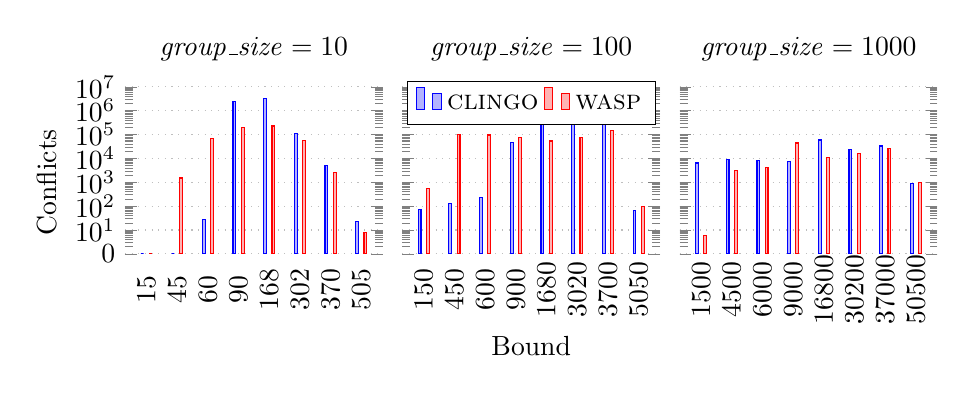
\begin{tikzpicture}
		\begin{axis}[
			xtick=data,
			xticklabels={$15$, $45$, $60$, $90$, $168$, $302$, $370$, $505$},
			ylabel={Conflicts},
            xlabel={},
            %xlabel={Asse x: bound/somma totale dei gruppi ($\mathit{bnd}_\sigma/\sum_{s \in S}{\max_{(w : \ell\ [s]) \in \sigma}w}$) per i diversi valori di $|\mathit{lits}_\sigma|_s|$},
            major x tick style=transparent,
			ybar,
			ymode=log,
			ymin=0.1,
			ymax=10000000,
			ytick={1, 10, 100, 1000, 10000, 100000, 1000000, 10000000},
			yticklabels={0, $10^1$, $10^2$, $10^3$, $10^4$, $10^5$, $10^6$, $10^7$},
			x axis line style={opacity=0},
            x tick label style={rotate=90, anchor=center},
			xtick=data,
			ymajorgrids=true,
			bar width=1pt,
			grid style=dotted,
			nodes near coords,
			scale only axis,
			point meta=explicit symbolic,
			% legend columns=-1,
			% legend pos=north east,
			height=0.2\textwidth,
			width=0.27\textwidth,
			name=plot1,
			title={$\mathit{group\_size} = 10$}
			]
			
			\addplot  coordinates {(0,1) (1,1) (2,27) (3, 2453921) (4, 3207378) (5, 112327) (6, 4845) (7, 22)};
            \addplot  coordinates {(0,1) (1,1506) (2,70594) (3, 194496) (4, 228698) (5, 58368) (6, 2492) (7, 8)};
			\legend{}
		\end{axis}	
		\begin{axis}[
			xtick=data,
			xticklabels={$150$, $450$, $600$, $900$, $1680$, $3020$, $3700$, $5050$},
			ylabel={},
            xlabel={Bound},
            %xlabel={Asse x: bound/somma totale dei gruppi ($\mathit{bnd}_\sigma/\sum_{s \in S}{\max_{(w : \ell\ [s]) \in \sigma}w}$) per i diversi valori di $|\mathit{lits}_\sigma|_s|$},
            major x tick style=transparent,
			ybar,
			ymode=log,
			ymin=0.1,
			ymax=10000000,
			ytick={1, 10, 100, 1000, 10000, 100000, 1000000, 10000000},
			yticklabels={},
			x axis line style={opacity=0},
            x tick label style={rotate=90, anchor=center},			
			xtick=data,
			ymajorgrids=true,
			bar width=1pt,
			grid style=dotted,
			nodes near coords,
			scale only axis,
			point meta=explicit symbolic,	
            legend columns=-1,
			% legend pos=north,
            legend style={at={(0.5,1.03)},anchor=north},
            height=0.2\textwidth,
			width=0.27\textwidth,
			name=plot2,
            at=(plot1.right of south east), anchor=left of south west,
			title={$\mathit{group\_size} = 100$}
			]
			
			\addplot  coordinates {(0,74) (1,124) (2,232) (3, 47209) (4, 263569) (5, 370134) (6, 476627) (7, 64)};
            \addplot  coordinates {(0,549) (1,100607) (2,95725) (3, 71962) (4, 53629) (5, 76733) (6, 152531) (7, 98)};	
            \legend{\textsc{clingo},\textsc{wasp}}
		\end{axis}
        \begin{axis}[
			xtick=data,
			xticklabels={$1500$, $4500$, $6000$, $9000$, $16800$, $30200$, $37000$, $50500$},
			ylabel={},
            xlabel={},
            %xlabel={Asse x: bound/somma totale dei gruppi ($\mathit{bnd}_\sigma/\sum_{s \in S}{\max_{(w : \ell\ [s]) \in \sigma}w}$) per i diversi valori di $|\mathit{lits}_\sigma|_s|$},
            major x tick style=transparent,
			ybar,
			ymode=log,
			ymin=0.1,
			ymax=10000000,
			ytick={1, 10, 100, 1000, 10000, 100000, 1000000, 10000000},
			yticklabels={},
			x axis line style={opacity=0},
			x tick label style={rotate=90, anchor=center},
			xtick=data,
            ymajorgrids=true,
			bar width=1pt,
			grid style=dotted,
			nodes near coords,
			scale only axis,
			point meta=explicit symbolic,            
			height=0.2\textwidth,
			width=0.27\textwidth,
			name=plot3,
            at=(plot2.right of south east), anchor=left of south west,
			title={$\mathit{group\_size} = 1000$}            
			]
			
			\addplot  coordinates {(0,6397) (1,8907) (2,8253) (3, 7461) (4, 59024) (5, 22660) (6, 33102) (7, 855)};
            \addplot  coordinates {(0,6) (1,3004) (2,4112) (3, 44378) (4, 10811) (5, 15519) (6, 25730) (7, 998)};									
		\end{axis}        
	\end{tikzpicture}
    \caption{
        Number of conflicts on synthetic AMOSUM constraints comprising 10 groups of varying size and bound.
        For each $\mathit{group\_size}$ there are four satisfiable instances (the first four bounds) and four unsatisfiable instances (the last four bounds).
        \textsc{amowasp} is not reported in the plots because it solves all tested instances in this benchmark without raising any conflict.
    }
    \label{fig:resultssynthetic}
\end{figure*}

The results obtained for GC and K are summarized in Figures~\ref{fig:graphcoloringknapsack}-~\ref{fig:scatter}.
As a first observation, \textsc{clingo} proves to be more efficient than \textsc{wasp} in both benchmarks.
As highlighted in SB, the branching heuristic of \textsc{clingo} is more effective than the one of \textsc{wasp}.
However, the inferences made by \textsc{amowasp} completely fulfil the gap related to the heuristic, and, in fact, \textsc{amowasp} achieves the best performance.
Regarding GC, \textsc{amowasp} successfully solves 72 instances, surpassing \textsc{clingo} and \textsc{wasp}, which solve 53 and 18 instances, respectively.
We additionally observe that the advantage of \textsc{amowasp} is particularly evident in instances with $\alpha = 0.75$, where it outperforms \textsc{clingo} and \textsc{wasp} by solving 48 and 60 more instances, respectively. However, for $\alpha = 0.15$ and $\alpha = 0.45$, the Python implementation introduces overhead, leading to comparatively poorer performance.
%
As for K, \textsc{amowasp} successfully solves 76 instances, outperforming both \textsc{clingo} and \textsc{wasp}, which solve 48 and 12 instances, respectively.
We additionally observe that \textsc{amowasp} consistently outperforms \textsc{wasp} across all instance categories,
solving 17, 25, 13, and 9 more instances of categories T1, T2, T3, and T4, respectively. 
In comparison to \textsc{clingo}, \textsc{amowasp} exhibits slightly poorer performance on T1 
instances, where \textsc{clingo} solves one more instance. However, 
it demonstrates better performance on the other instances, solving 16, 4, and 9 more T2, T3 and T4 instances, respectively.

\begin{figure*}[h]
    \begin{tikzpicture}[scale=0.7]
    \pgfkeys{%
        /pgf/number format/set thousands separator = {}}
    \begin{axis}[
    scale only axis
    , xlabel={Solved instances}
    , ylabel={Execution time (s)}
    , xmin=0, xmax=80
    , ymin=0, ymax=1220
    , legend style={at={(0.18,0.96)},anchor=north,fill=none}
    , legend columns=1
    , width=0.65\textwidth
    , height=0.40\textwidth
    , ytick={0,200,400,600,800,1000,1200}
    , major tick length=2pt
    , title= {Graph Coloring}
    ]
    \addplot [mark size=3pt, color=blue, mark=triangle*] [unbounded coords=jump] table[col sep=semicolon, y index=1] {./graphcoloringcactus.csv}; 
    \addlegendentry{\textsc{clingo}}
    
    \addplot [mark size=3pt, color=red, mark=triangle] [unbounded coords=jump] table[col sep=semicolon, y index=2] {./graphcoloringcactus.csv}; 
    \addlegendentry{\textsc{wasp}}
    
    \addplot [mark size=3pt, color=black, mark=o] [unbounded coords=jump] table[col sep=semicolon, y index=3] {./graphcoloringcactus.csv}; 
    \addlegendentry{\textsc{amowasp}}    
    \end{axis}
    \end{tikzpicture}%
    \hfill
    \begin{tikzpicture}[scale=0.7]
    \pgfkeys{%
        /pgf/number format/set thousands separator = {}}
    \begin{axis}[
    scale only axis
    , xlabel={Solved instances}
    , xmin=0, xmax=80
    , ymin=0, ymax=1220
    , legend style={at={(0.18,0.96)},anchor=north,fill=none}
    , legend columns=1
    , width=0.65\textwidth
    , height=0.40\textwidth
    , ytick={0,200,400,600,800,1000,1200}
    , yticklabels = {}
    , major tick length=2pt
    , title= {Knapsack}
    ]
    \addplot [mark size=3pt, color=blue, mark=triangle*] [unbounded coords=jump] table[col sep=semicolon, y index=1] {./knapsackcactus.csv}; 
    \addlegendentry{\textsc{clingo}}
    
    \addplot [mark size=3pt, color=red, mark=triangle] [unbounded coords=jump] table[col sep=semicolon, y index=2] {./knapsackcactus.csv}; 
    \addlegendentry{\textsc{wasp}}
    
    \addplot [mark size=3pt, color=black, mark=o] [unbounded coords=jump] table[col sep=semicolon, y index=3] {./knapsackcactus.csv}; 
    \addlegendentry{\textsc{amowasp}}    
    \end{axis}
    \end{tikzpicture}%
    \caption{
        Number of solved instances ($x$-axis) within a time limit ($y$-axis) for Graph Coloring (left) and Knapsack (right).
        %In particular, observe that \textsc{amowasp} solved XX and XX instances within 200 seconds of computation, while \textsc{wasp} and \textsc{clingo} only XX and XX, respectively.
    }\label{fig:graphcoloringknapsack}          
\end{figure*}


\begin{figure}
    \centering
\begin{tikzpicture}[scale=0.7]
    \pgfkeys{%
        /pgf/number format/set thousands separator = {}}
    \begin{axis}[
    scale only axis
    , legend style={at={(0.75,0.3)}, anchor=south, align=left}
    , legend cell align=left
    , xlabel={\textsc{wasp}}
    , ylabel={\textsc{amowasp}}
    , width=0.25\textwidth
    , height=0.25\textwidth
    , xmin=0, xmax=1200
    , ymin=0, ymax=1200
    , xtick={300,600,900,1200}
    , xticklabels={300,600,900,1200}
    , ytick={300,600,900,1200}
    , yticklabels={300,600,900,1200}
    , major tick length=2pt
    , title={Graph Coloring}
    ]
    \addplot [mark size=3pt, only marks, color=blue, mark=star] [unbounded coords=jump] table[col sep=semicolon, x index=4, y index=5] {graphcoloringscatter15.csv};     
    \addlegendentry{$\alpha = 0.15$}

    \addplot [mark size=3pt, only marks, color=darkorange, mark=o] [unbounded coords=jump] table[col sep=semicolon, x index=4, y index=5] {graphcoloringscatter45.csv};
    \addlegendentry{$\alpha = 0.45$}

    \addplot [mark size=3pt, only marks, color=darkgreen, mark=triangle] [unbounded coords=jump] table[col sep=semicolon, x index=4, y index=5] {graphcoloringscatter75.csv};     
    \addlegendentry{$\alpha = 0.75$}

    \addplot [color=red, dashed] [unbounded coords=jump] coordinates {(0,0) (1200,1200)}; 
    \end{axis}
\end{tikzpicture}
\begin{tikzpicture}[scale=0.7]
    \pgfkeys{%
        /pgf/number format/set thousands separator = {}}
    \begin{axis}[
    scale only axis
    , legend style={at={(0.75,0.3)}, anchor=south, align=left}
    , legend cell align=left
    , xlabel={\textsc{clingo}}
    %, ylabel={\textsc{amowasp}}
    , width=0.25\textwidth
    , height=0.25\textwidth
    , xmin=0, xmax=1200
    , ymin=0, ymax=1200
    , xtick={300,600,900,1200}
    , xticklabels={300,600,900,1200}
    , ytick={300,600,900,1200}
    , yticklabels={}
    , major tick length=2pt
    , title={Graph Coloring}
    ]
    \addplot [mark size=3pt, only marks, color=blue, mark=star] [unbounded coords=jump] table[col sep=semicolon, x index=3, y index=5] {graphcoloringscatter15.csv};     
    \addlegendentry{$\alpha = 0.15$}

    \addplot [mark size=3pt, only marks, color=darkorange, mark=o] [unbounded coords=jump] table[col sep=semicolon, x index=3, y index=5] {graphcoloringscatter45.csv};
    \addlegendentry{$\alpha = 0.45$}

    \addplot [mark size=3pt, only marks, color=darkgreen, mark=triangle] [unbounded coords=jump] table[col sep=semicolon, x index=3, y index=5] {graphcoloringscatter75.csv};     
    \addlegendentry{$\alpha = 0.75$}

    \addplot [color=red, dashed] [unbounded coords=jump] coordinates {(0,0) (1200,1200)}; 
    \end{axis}
\end{tikzpicture}


\begin{tikzpicture}[scale=0.7]
    \pgfkeys{%
        /pgf/number format/set thousands separator = {}}
    \begin{axis}[
    scale only axis
    , legend style={at={(0.75,0.3)}, anchor=south, align=left}
    , legend cell align=left
    , xlabel={\textsc{wasp}}
    , ylabel={\textsc{amowasp}}
    , width=0.25\textwidth
    , height=0.25\textwidth
    , xmin=0, xmax=1200
    , ymin=0, ymax=1200
    , xtick={300,600,900,1200}
    , xticklabels={300,600,900,1200}
    , ytick={300,600,900,1200}
    , yticklabels={300,600,900,1200}
    , major tick length=2pt
    , title={Knapsack}
    ]
    \addplot [mark size=3pt, only marks, color=blue, mark=star] [unbounded coords=jump] table[col sep=semicolon, x index=4, y index=5] {knapsackscatter-type1.csv};     
    \addlegendentry{T1}

    \addplot [mark size=3pt, only marks, color=darkorange, mark=o] [unbounded coords=jump] table[col sep=semicolon, x index=4, y index=5] {knapsackscatter-type2.csv};
    \addlegendentry{T2}

    \addplot [mark size=3pt, only marks, color=darkgreen, mark=triangle] [unbounded coords=jump] table[col sep=semicolon, x index=4, y index=5] {knapsackscatter-type3.csv};     
    \addlegendentry{T3}
    
    \addplot [mark size=3pt, only marks, color=darkviolet, mark=square] [unbounded coords=jump] table[col sep=semicolon, x index=4, y index=5] {knapsackscatter-type4.csv};     
    \addlegendentry{T4}

    \addplot [color=red, dashed] [unbounded coords=jump] coordinates {(0,0) (1200,1200)}; 
    \end{axis}
\end{tikzpicture}
\begin{tikzpicture}[scale=0.7]
    \pgfkeys{%
        /pgf/number format/set thousands separator = {}}
    \begin{axis}[
    scale only axis
    , legend style={at={(0.75,0.3)}, anchor=south, align=left}
    , legend cell align=left
    , xlabel={\textsc{clingo}}
    %, ylabel={\textsc{amowasp}}
    , width=0.25\textwidth
    , height=0.25\textwidth
    , xmin=0, xmax=1200
    , ymin=0, ymax=1200
    , xtick={300,600,900,1200}
    , xticklabels={300,600,900,1200}
    , ytick={300,600,900,1200}
    , yticklabels={}
    , major tick length=2pt
    , title={Knapsack}
    ]
    \addplot [mark size=3pt, only marks, color=blue, mark=star] [unbounded coords=jump] table[col sep=semicolon, x index=3, y index=5] {knapsackscatter-type1.csv};     
    \addlegendentry{T1}

    \addplot [mark size=3pt, only marks, color=darkorange, mark=o] [unbounded coords=jump] table[col sep=semicolon, x index=3, y index=5] {knapsackscatter-type2.csv};
    \addlegendentry{T2}

    \addplot [mark size=3pt, only marks, color=darkgreen, mark=triangle] [unbounded coords=jump] table[col sep=semicolon, x index=3, y index=5] {knapsackscatter-type3.csv};     
    \addlegendentry{T3}
    
    \addplot [mark size=3pt, only marks, color=darkviolet, mark=square] [unbounded coords=jump] table[col sep=semicolon, x index=3, y index=5] {knapsackscatter-type4.csv};     
    \addlegendentry{T4}

    \addplot [color=red, dashed] [unbounded coords=jump] coordinates {(0,0) (1200,1200)}; 
    \end{axis}
\end{tikzpicture}
    \caption{
        Instance-by-instance comparison on the execution time (in seconds) required to solve Graph Coloring and Knapsack.
        (Timeouts normalized to 1200 seconds.)
        Points below the red dashed line are instances in which \textsc{amowasp} is faster than the compared system.
    }\label{fig:scatter}
\end{figure}

To sum up, \textsc{amowasp} outperforms \textsc{wasp} thanks to the technique presented in this paper, 
as \textsc{amowasp} is powered by \textsc{wasp} and thus inherits all of its heuristic parameters.


\chapter{Related Work}
\label{sec:rw}
In this work, AMOSUM constraints have been incorporated into the (propositional) language of ASP. 
However, AMOSUMs can be integrated into any logic-based formalism that extends propositional logic, 
such as SMT \cite{DBLP:journals/jacm/NieuwenhuisOT06} and CSP \cite{DBLP:journals/eor/BrailsfordPS99}. 
From a computational perspective, there are two primary methods to enhance the capabilities of logic-based languages: 
the \textit{propagator-based} approach and the \textit{translation-based} approach, as discussed below.

Solvers that utilize the \emph{propagator-based} approach implement specialized algorithms 
to extend assignments with literals that must be true (Section ~\ref{sec:bg-SM}). 
The method used to handle AMOSUM constraints in this work (Section ~\ref{sec:amo:syntax_semantics}) falls within this category. 
In the existing literature, the state-of-the-art system \textsc{clingo} \cite{DBLP:journals/tplp/GebserKKS19} employs a 
hybrid approach for managing programs with aggregates \cite{DBLP:conf/iclp/GebserKKS09}. Aggregates containing a limited 
number of literals are transformed into regular rules using a translation-based approach, with the threshold for the number 
of literals being adjustable via the command-line interface. Other aggregates, including those representing AMO constraints, 
are handled by the propagator described in Section ~\ref{sec:amo:propagator}.
A similar approach is also implemented in \textsc{idp} \cite{Denecker2010DPLLAggAE,DBLP:journals/ngc/0001JCJBD16} 
and \textsc{wasp} \cite{DBLP:journals/tplp/AlvianoDM18}. 
Additionally, both \textsc{clingo} and \textsc{wasp} 
provide external Python-based interfaces for defining custom 
propagators ~\cite{DBLP:journals/algorithms/CabalarFSW23,DBLP:journals/tplp/DodaroR20}. 
The propagator described in Section~\ref{sec:amo:propagator} is implemented using the Python interface of \textsc{wasp}.

Translation-based approaches involve compiling aggregates into alternative constructs. 
In the context of ASP, the similarities between aggregates and pseudo-Boolean constraints have 
led to the adoption of certain pseudo-Boolean constraint compilations into clauses \cite{DBLP:conf/sara/AavaniMT13}. 
In the context of ASP solvers, many of these translation techniques are integrated into tools like \textsc{lp2sat} and 
\textsc{lp2normal} \cite{DBLP:conf/jelia/BomansonGJ14,DBLP:conf/lpnmr/BomansonJ13}. The former generates CNF formulas, 
while the latter produces normal rules. Another translation-based method is employed by 
\textsc{cmodels} \cite{DBLP:conf/lpnmr/LierlerM04,DBLP:journals/jar/GiunchigliaLM06,DBLP:journals/amai/GiunchigliaLM08}, 
which translates aggregates into nested logic programs \cite{DBLP:journals/tplp/FerrarisL05}.
Finally, for AMO constraints, translation-based approaches provide several encoding options, 
including pairwise (binomial), binary (bitwise), commander, product, sequential counter, 
and bimander encodings. A recent comparison of these encodings can be found in \cite{DBLP:conf/sma2/NguyenNKB20}. 
It is worth noting that the AMOSUM propagator introduced in this article can be integrated with AMO constraint 
compilers by substituting the first inference rule specified in Section~\ref{sec:amo:inference_rules} with the compiled clauses.

\chapter{Conclusion}
\newpage
\printbibliography
\end{document}